\documentclass[11pt,twocolumn]{article}
\usepackage[margin=0.8in]{geometry}                % See geometry.pdf to learn the layout options. There are lots.
\geometry{letterpaper}                   % ... or a4paper or a5paper or ... 
%\geometry{landscape}                % Activate for for rotated page geometry
%\usepackage[parfill]{parskip}    % Activate to begin paragraphs with an empty line rather than an indent
\usepackage{color}
\definecolor{myblue}{rgb}{0.0, 0.0, 0.85}
\usepackage[breaklinks=true, colorlinks=true, linkcolor=red, urlcolor=myblue, citecolor=black]{hyperref}
\urlstyle{rm}
\usepackage{amsmath}
\usepackage{mathptmx}
\usepackage{graphicx}
\usepackage{amssymb}
\usepackage{epstopdf}
\usepackage{sidecap}
\usepackage{authblk}
\usepackage{booktabs}
\usepackage[font=small,labelfont=bf]{caption}
\DeclareGraphicsRule{.tif}{png}{.png}{`convert #1 `dirname #1`/`basename #1 .tif`.png}
\usepackage{enumitem}
\setlist[itemize]{noitemsep}
\setlist[enumerate]{noitemsep}

\def\bfr{\bf\color{red}}
\def\geohub{{\tt geohub}}
\def\Count{count}
\def\ntracts{39}
\def\nprof{9}
\def\nvol{30}
\def\resp{respectively}

\title{\bf
	Results of the 2021 Greater Hollywood Volunteer Homeless Count
	}
\author[1,2,3,$\dagger$]{Louis Abramson}
\author[4]{Brian Kohan}
\author[1,5]{Jackie Vorhauer}
\author[1,6]{Heather Carmichael}
\author[1,7]{Helen Eigenberg}
\author[1,8]{Stephen Fiechter}
\author[1]{David Gordon}
\author[9]{Courtney Kanagi}
\author[1,10]{Emily Uyeda Kantrim}
\author[9]{Guido Merkens}
\author[1,10]{Arnali Ray}
\author[5]{Elyse Schwartz}
\author[1,5]{Douglas Walker}
\author[1]{Kerry Morrison}
\affil[1]{\it \small Hollywood 4WRD Homelessness Coalition, 6255 Sunset Blvd, Ste 150, Los Angeles, CA 90028}
\affil[2]{\it Central Hollywood Neighborhood Council, PO Box 93907, Los Angeles, CA 90093}
\affil[3]{\it Carnegie Observatories, 813 Santa Barbara St, Pasadena, CA 91101}
\affil[4]{\it SELAH Neighborhood Homeless Coalition, \bf address}
\affil[5]{\it The Center at Blessed Sacrament, 6636 Selma Ave, Los Angeles, CA 90028}
\affil[6]{\it My Friend's Place, 5850 Hollywood Blvd, Los Angeles, CA 90028}
\affil[7]{\it Hang Out Do Good, \bf address}
\affil[8]{\it People Assisting The Homeless, 340 N Madison Ave, Los Angeles, CA 90004}
\affil[9]{\it The Hollywood Partnership, 6562 Hollywood Blvd, Los Angeles, CA 90028}
\affil[10]{\it Mid City West Community Council, 644 N Fuller Ave, PMB 7059, Los Angeles, CA 90036}
\affil[$\dagger$]{Corresponding author; \href{mailto:labramson.chnc@gmail.com}{labramson.chnc@gmail.com}}

\date{\vspace{-1em}Draft: \today}                                           % Activate to display a given date or no date

\begin{document}
\maketitle

\begin{abstract}

Data from February 25, 2021 censuses of Hollywood and East Hollywood shows that 
unsheltered homelessness has fallen in those communities by $11\%\pm9\%$ and 
$15\%\pm12\%$, \resp, compared to the 2020 LAHSA Point-In-Time (PIT) count (90\% CI). 
A 30\% drop in individuals seen on the street drives this change, reducing the number of identified 
persons and dwellings in about a third of census tracts. Unsheltered living is thus likely to have 
declined quantitatively even if the average occupancy of, e.g., tents is updated. Simultaneously, 
however, 13\% of tracts saw at least a doubling in street dwellings. This trend may contribute to 
qualitative perceptions that the state of homelessness has worsened over the past year, which---given 
COVID-related reductions in health, hygiene, and social support services---are also likely to be accurate.
Coordinated Entry System data will reveal whether homelessness has declined in toto or if 
government initiatives reduced only the portion of people living unsheltered in Greater Hollywood.

\end{abstract}

\section{Introduction}
\label{sec:intro}

The Los Angeles Homelessness Services Authority (LAHSA) conducts an annual Point In Time (PIT) 
census of the unhoused population of Los Angeles County. These data inform programmatic
funding levels, educate residents, undergird legislative efforts, and shape the day-to-day practices of 
professional and volunteer service providers. 

As the official assessment of the scope of one of the most pressing humanitarian issues of our time, 
the LAHSA Count is invaluable. However, due to disruptions from COVID-19, the unsheltered portion 
of the 2021 PIT count was cancelled. Since 70\% of LA's unhoused residents were unsheltered as of 
2020, absent additional efforts, this cancellation would substantially erode our understanding of 
the state of homelessness following an unprecedented year of economic disruptions and governmental 
interventions---both of which may have significantly affected the number of unhoused LA County residents.

Greater Hollywood is an epicenter of the homelessness crisis. According to the 2020 Count, the 
Hollywood and East Hollywood Communities were home to 2203 unhoused residents, 1714 of whom 
(78\%) were unsheltered. This figure corresponds to roughly 
\href{https://www.lahsa.org/data?id=45-2020-homeless-count-by-community-city}
{5\% of LA's homeless population} concentrated in an area with 
\href{https://geomap.ffiec.gov/FFIECGeocMap/GeocodeMap1.aspx}{3.5\% of its total population}. 
In some areas, 1-in-25 Hollywood residents are unhoused compared to 1-in-100 citywide.

\begin{figure*}
	\centering
	\includegraphics[width=0.9\linewidth]{countMap}
	\caption{The 2021 volunteer \Count\ covered Greater Hollywood, comprising the 
			officially recognized LAHSA Hollywood and East Hollywood Continua
			of Care. The former stretches from Laurel Canyon Blvd to Western Ave,
			the latter from Western to Hoover Ave. Hollywood is bounded to the north
			and south respectively by Franklin	and Melrose Aves, with East Hollywood
			bounded by Hollywood Blvd and Beverly Ave. Hollywood comprises
			21 census tracts; East Hollywood 18.}
	\label{fig:map}	
\end{figure*}

While the above statistics are tragic, Hollywood is also marked by large and increasingly formalized
coalitions of service providers, business leaders, residents, and governmental entities dedicated to 
humanely ending homelessness in their community. Given the capacity of the above organizations and 
individuals, and given the importance of the annual PIT count in educating local residents, funders, and
legislators, Hollywood decided to proceed as a collective with an unsponsored grassroots PIT \Count\
in 2021.

This document describes the methodology and findings of that \Count, which took place on Thursday, 
February 25, 2021. Section \ref{sec:procedure} describes the volunteer training, data acquisition, 
and analysis protocols. Section \ref{sec:results} presents estimates of the unsheltered 
populations in the Hollywood and East Hollywood Communities and contextualizes those findings in 
terms of the 2020 LAHSA results. Section \ref{sec:discussion} describes cross-checks, provides some 
interpretation, highlights areas for further study, and reveals where quantitive findings may drive 
qualitative impressions among residents as to the ``felt'' state of the crisis. Section \ref{sec:summary} 
summarizes. Additional information can be found in the Appendix, including a table of tract-level 
results in each of the survey's 39 US Census tracts. All data are available at {\bfr website}.

\section{Methodology}
\label{sec:procedure}
%
%The \Count\ took place on 25 February 2021 circa at 7.00 PM. This timing corresponds to one month 
%after and four hours before the official event would have occurred. Beyond those choices, our program 
%adhered as closely as possible to the official LAHSA 2020 PIT data collection and analysis protocols. 
%
%The \Count\ was launched from The Center at Blessed Sacrament (``The Center''), a major service 
%provider in Hollywood, at 6636 Selma Ave. All volunteer teams reported and returned to this 
%location as they would to a LAHSA community hub in past years, but, as COVID precautions, 
%training was performed remotely in the week preceding the count and volunteers never left their 
%vehicles.

\subsection{Data Acquisition}
\label{sec:acquisition}

The \Count\ was based out of The Center at Blessed Sacrament (``The Center''), a major service 
provider in Hollywood. All volunteers reported and returned to this location as they would a LAHSA 
community hub in the past. Training was performed offsite, however, volunteers
never left their vehicles, and the majority of surveying occurred between 7:00 PM and 10:00 PM.

The \Count\ covered the \ntracts\ US Census tracts constituting the LAHSA-defined 
\href{https://www.lahsa.org/data?id=45-2020-homeless-count-by-community-city}{Hollywood 
and East Hollywood Communities} (21 and 18 tracts, \resp). It did not recognize census 
tract ``splits''---e.g., ``1905.10a''---which modified of the definition of Hollywood to include 
all of tract 1905.10 and East Hollywood to include all of tract 1913.01. Since 2016, tract 1905.10b has 
never hosted more than 7 unsheltered people abd 1913.01a never more than 15 people. As such,
these modifications do not affect community-level results significantly.
%Sections \ref{sec:results} and \ref{sec:discussion} discuss community-level results with 
%tract-level tallies provided in the Appendix. Results for Greater Hollywood are not directly comparable 
%to any official service geography but are available upon request. 
Figure \ref{fig:map} shows the \Count\ footprint.

All tracts were vetted by outreach professionals from The Center prior to assignment. Tracts 
deemed especially challenging---e.g., due to their proximity to freeway onramps/peripheries---were 
reserved for professional counting teams. Vetting produced \nprof\ such tracts, which were surveyed 
by personnel from The Center and Covenant House circa 3:00 PM on 25 February. The remaining \nvol\ 
tracts were divided among the volunteer vehicle-based teams and surveyed beginning at 7.00 PM. With 
the exception of one tract in East Hollywood, teams were restricted to one or the other community, 
making the community-level results nearly independent. Cross-comparisons therefore serve as data 
quality indicators (Section \ref{sec:discussion}). Table \ref{tbl:tractStats} records which tract was 
counted by which kind of team. 

Thirty-two volunteer teams participated in the \Count, which was limited to existing ``pods'' of two 
to three people to minimize the possibility of COVID transmission. Singlet volunteers were admitted 
but remained on-site to assist with traffic control and material distribution. All participants wore 
personal protective equipment and maintained social distancing when appropriate.

Counting followed 2020 LAHSA PIT protocols to the greatest extent possible. Each volunteer team 
was assigned two tracts and comprised at least a Driver and a Counter. Three-person teams 
included a Navigator, as well. If present, the Navigator directed the Driver while the Counter tallied 
unhoused individuals/dwellings. In two-person teams, the Counter doubled as the Navigator. Training 
emphasized techniques aimed at reducing Counters' cognitive loads to minimize counting errors, e.g., 
covering interior streets in a serpentine pattern before circling the tract border. Teams were instructed 
to count both sides of interior streets but only interior sides of border streets as described in the official 
2020 PIT training video.

All teams were deployed to their tracts by roughly 7:30 PM and returned by 9:55 PM.

Upon arriving at The Center, organizers provided each team a clipboard containing:
\begin{itemize}
	\item two tract maps;
	\item two tally sheets;
	\item one 1-page training summary with a contact number for field issues.
\end{itemize}
See Appendix for examples.

The tally sheets were the data acquisition tool. These contained separate columns for each of the 
nine categories of unhoused individuals/dwellings recognized in the 2020 LAHSA PIT count: 
\begin{enumerate}
	\item adults (ages $\geq$25);
	\item transition age youths (``TAY,'' 18--24);
	\item unaccompanied minors;
	\item families (at least one adult with at least one minor); 
	\item cars;
	\item vans;
	\item RVs;
	\item tents;
	\item makeshift structures.
\end{enumerate}
The dwelling classes---Items 5--9---are treated differently than the individual classes in the analysis,
and are hereafter referred to by their acronym, ``CVRTM,'' when appropriate. Adults+TAY may
also be combined into ``Persons'' (P). No families or unaccompanied minors were identified.\footnote{
One potential unaccompanied minor was reported in tract 1912.01 but could not be confirmed by outreach
personnel dispatched to that location. One potential family was also reported dwelling in a van in
tract 1899.05 that could also not be confirmed. The upper limits for these categories (3 each at 95\%
confidence) capture this uncertainty, but their raw counts are set to zero.}

Upon returning,  Counters verbally read their results to organizers, who entered them into a google 
form. The organizer read back the results for confirmation before submitting the form and recovering the
hand-written tallies from the volunteers. 
%Volunteer email addresses were also retained for follow-up. 

Once all materials were collected, the organizers convened to cross-check the electronic records---a
google sheet automatically generated by the google form responses---with the physical tally sheets and 
identify any uncounted areas. None of the latter were found that required follow-up. Any disagreement 
between electronic and paper references was cross-checked and corrected to the paper tally. All 
data are available at {\bfr website}.

Given turnout, every volunteer tract was counted by at least two teams, with four tracts counted in 
triplicate. Beyond increasing the accuracy of the count, repeat measurements aid the understanding of 
counting errors (Sections \ref{sec:dupes}) and provide robustness---one tally was uninterpretable, leaving 
only the result from the other team on that tract.

All told, the data set comprises 37 pair-wise volunteer measurements---29 duplicates + 
4 triplicates (=8 additional pairs)---one singly-counted volunteer tract estimate, and nine unique 
professional assessments. The latter comprise about 20\% of tracts in both communities and roughly 
43\% of the total individuals and dwellings counted. Year-on-year trends are consistent between
volunteer- and professionally counted tracts (Section \ref{sec:discussion}). 
%The largest increase was observed by volunteers, the largest
%decrease by professionals.%; both tracts are located in E.~Hollywood.

\begin{table}[t!]
\caption{Tract-level Unsheltered Population Summary}
\resizebox{\linewidth}{!}{%
\begin{tabular}{cccccc}
\toprule
Tract & Community & Counter$^{\rm a}$ & Passes$^{\rm b}$ & Median Est. & 90\% CI \\ 
 & & & & [people] & [people] \\ \cmidrule{1-6}
1898.00 & Hollywood & Vol & 3 & 6 & 0--15 \\
1899.02 & Hollywood & Vol & 3 & 18 & 12--24 \\
1899.03 & Hollywood & Vol & 2 & 0 & 0--12 \\
1899.04 & Hollywood & Vol & 2 & 18 & 11--25 \\
1899.05 & Hollywood & Vol & 2 & 19 & 9--30 \\
1901.00 & Hollywood & Vol & 2 & 88 & 75--102 \\
1902.01 & Hollywood & Vol & 2 & 21 & 13--29 \\
1902.02 & Hollywood & Vol & 2 & 30 & 20--40 \\
1903.01 & Hollywood & Pro & 1 & 74 & 54--96 \\
1905.10 & Hollywood & Pro & 1 & 34 & 22--46 \\
1905.20 & E.~Hollywood & Vol & 2 & 12 & 6--18 \\
1907.00 & Hollywood & Vol & 2 & 110 & 93--127 \\
1908.01 & Hollywood & Vol & 2 & 63 & 50--76 \\
1908.02 & Hollywood & Pro & 1 & 71 & 54--90 \\
1909.01 & Hollywood & Pro & 1 & 55 & 39--71 \\
1909.02 & Hollywood & Vol & 3 & 6 & 0--17 \\
1910.00 & Hollywood & Pro & 1 & 169 & 140--201 \\
1911.10 & E.~Hollywood & Vol & 2 & 9 & 2--15 \\
1911.20 & E.~Hollywood & Pro & 1 & 66 & 48--85 \\
1912.01 & E.~Hollywood & Vol & 2 & 55 & 44--68 \\
1912.03 & E.~Hollywood & Vol & 2 & 26 & 14--38 \\
1912.04 & E.~Hollywood & Vol & 2 & 6 & 0--16 \\
1913.01 & E.~Hollywood & Vol & 2 & 31 & 22--42 \\
1913.02 & E.~Hollywood & Vol & 2 & 23 & 15--30 \\
1914.10 & E.~Hollywood & Vol & 2 & 20 & 13--28 \\
1914.20 & E.~Hollywood & Vol & 2 & 24 & 16--32 \\
1915.00 & E.~Hollywood & Vol & 2 & 29 & 21--38 \\
1916.10 & E.~Hollywood & Pro & 1 & 48 & 31--68 \\
1916.20 & E.~Hollywood & Pro & 1 & 17 & 6--30 \\
1917.10 & Hollywood & Vol & 2 & 21 & 14--29 \\
1917.20 & Hollywood & Vol & 3 & 21 & 12--31 \\
1918.10 & Hollywood & Vol & 2 & 24 & 14--34 \\
1918.20 & Hollywood & Vol & 2 & 16 & 10--23 \\
1919.01 & Hollywood & Vol & 2 & 60 & 49--72 \\
1925.10 & E.~Hollywood & Vol & 2 & 12 & 4--21 \\
1925.20 & E.~Hollywood & Vol & 1 & 14 & 1--28 \\
1926.10 & E.~Hollywood & Vol & 2 & 7 & 1--14 \\
1926.20 & E.~Hollywood & Vol & 2 & 18 & 9--26 \\
1927.00 & E.~Hollywood & Pro & 1 & 129 & 96--167\\
\cmidrule{1-6}
{\bf All} & & & {\bf 72}$^{\rm c}$ & {\bf 1494} & {\bf 1342--1657}
\\ \bottomrule
\end{tabular}
}
\caption*{$^{\rm a}$Volunteer vs.~professional surveyor; $^{\rm b}$independent 
		tract counts; $^{\rm c}$reflects one tally rejected during quality control.}
\label{tbl:tractStats}
\end{table}

\subsubsection{Volunteer Training}
\label{sec:training}

Teams underwent mandatory, $\sim$30 minute Zoom-based training sessions before arriving 
for the \Count. Each participant was also required to watch the official 2020 LAHSA PIT training 
video.% and sign participation waivers.

The training covered the motivation for the \Count, an overview of the survey geography, team roles, 
and examples of unhoused dwellings. Except in the case of people standing next to tents---as described 
in the 2020 LAHSA video---volunteers were instructed to count CVRTM and individuals separately 
and not to try to estimate how many people might live in or be associated with a specific dwelling. 
This ensured that results could be analyzed as a function of the CVRTM weights, which may change 
with future information.% (see Section \ref{sec:analysis}).

Volunteers were primed only with min/max estimates of tract-level individual+dwelling counts 
(``0--120'') and the likelihood of encountering unaccompanied minors or families (``very unlikely'')
or TAY (``some tracts especially in Hollywood''). These statements were informed by the 2020 LAHSA PIT 
results. No other prior was established. The training presentation is available 
at: \url{https://drive.google.com/file/d/1xFrtU26yjPuiUv9KHZ3Uj2_sAoT1ClGo/view?usp=sharing}.

\subsection{Data Analysis}
\label{sec:analysis}

The data form a $9\times73$ array containing the tract-level tallies for each unhoused 
individual/dwelling class. Data reduction involves simply averaging repeat counts of the same tract,
associating the latter with the Hollywood or East Hollywood community, and 
weighting by the CVRTM mean occupancies. We produce 10,000 realizations of the final dataset
incorporating random perturbations of the counts and weights according to their uncertainties 
(see below). The resulting final population inference is a $9\times10000\times39$ array that 
may be split and summed to provide aggregate, tract, or category-level population estimates and 
uncertainties.

Our baseline result incorporates the \href{https://www.lahsa.org/documents?id=4686-2020-greater-los-angeles-city-community-homelessness-report-service-planning-area-4.pdf}{2020 SPA-4/CD13 CVRTM weights}, 
which underpin the latest LAHSA \href{https://www.lahsa.org/documents?id=4686-2020-greater-los-angeles-city-community-homelessness-report-service-planning-area-4.pdf}
{Community Summaries}. However, we recognize that COVID-related activities such as tent 
distribution efforts may have changed these weights in reality. We cannot reassess all of them and 
encourage robust efforts to do so. However, at least one survey of tent-dwellers in Hollywood suggests 
the tent weight, $T$, has not changed significantly. We analyze the impact of adopting three other
reasonable CVRTM choices in Section \ref{sec:CVRTM} (Table \ref{tbl:weights}), but they do not 
significantly affect our findings.

%While an estimate of the underlying population, uncertainties in each visual count and weight 
%must be accounted for to understand how confident one can be that that estimate corresponds to
%the truth. We accomplish this by using Monte Carlo integration to construct the full probability
%distribution functions (PDFs) for the number of unsheltered people of each class in each tract.

% {\it These results will
%correspond to the most likely values for the respective quantities in any geography.} However,
%three uncertainties---one small and two large---complicate the interpretation of those sums. 
%We discuss these in Section \ref{sec:discussion}, but account for them as best we can using 
%Monte Carlo techniques to construct the full underlying probability distribution functions (PDFs) 
%for each class in each tract.
%
%All results discussed below derive from 10,000 Monte Carlo realizations of Item (5), above.
%

\subsubsection{Monte Carlo Population Inferences}
\label{sec:mc}

We wish to infer the true unsheltered population in Hollywood and East Hollywood as of 25 February. 
We do so by constructing probability density functions (PDFs) describing the likelihood of encountering 
a given number of unsheltered people in those communities as constrained by our PIT \Count\ data. 
To accomplish this, we must model three known uncertainties: (1) errors in the visual tallies, (2) deviations 
of the CVRTM weights from their quoted means, and (3) the intrinsic background rate of persons/dwellings
in areas in which none were actually sighted. Items (1) and (3) reflect how our PIT tally might change
if performed at a different (but comparable) time or by different teams. Item (2) reflects how the mean 
occupancy of CVRTM structures in our survey area might differ from the mean occupancy in the geography 
in which the weights were defined.

We model (1) and (2) as independent random draws from Gaussian distributions with standard 
deviations of $\sqrt{n}$ and $\sigma$, \resp, where $n$ is the raw PIT tally and $\sigma$ is the 
standard error on the respective CVRTM weight, $w$, quoted by LAHSA. As such, the $i$-th 
estimate of the true number, $N$, of people belonging to the $j$-th unsheltered class in any tract is:
\begin{multline}\label{eq:monte}
	N_{i,j} = \left[n_{j} + \mathcal{G}_{i}(0,\sqrt{n_{j}})\right]\times\max[\mathcal{G}_{i}(w_{j}, \sigma_{j}),1],
\end{multline}
where $\mathcal{G}(\mu,\Sigma)$ is a Gaussian random number with mean $\mu$ and standard deviation 
$\Sigma$. If more than one team counted a given tract, $n$ is replaced by the average of their tallies 
and the attendant counting error is divided by the square root of the number of teams. If no members
of the $j$-th unsheltered category were observed, $\sqrt{n_{j}}$ is replaced in the first term 
by that category's estimated background rate, $\sigma_{j}^{\rm bkg}$, which we discuss
in the next section.% \ref{sec:nulls}).

The final output probability distribution functions (PDFs) are based on 10,000 realizations of 
Equation \ref{eq:monte}. Weights for adults and TAY are fixed to unity, such that 
$(w,\sigma)\equiv(1,0)$ for all trials and uncertainties reflect only counting errors. One potential 
family and one potential unaccompanied minor were reported, but not confirmed. We therefore
set those entires to zero and infer only upper limits.

We place a floor on the CVRTM mean occupancies at 1 person per dwelling; i.e., we assume that the 
{\it mean} person does not own more than one dwelling. This is not to say no one may own more than 
one, just that such a statement is never representative. This choice induces a mild asymmetry in our 
global PDFs but does not significantly affect inferences.
%letting the mean occupancies reach 0 moves the baseline result down by 40 ppl over all of grtr Hwood.
%it's 0.4 sigma or in the IQR.

\begin{figure}[t]
\centering
	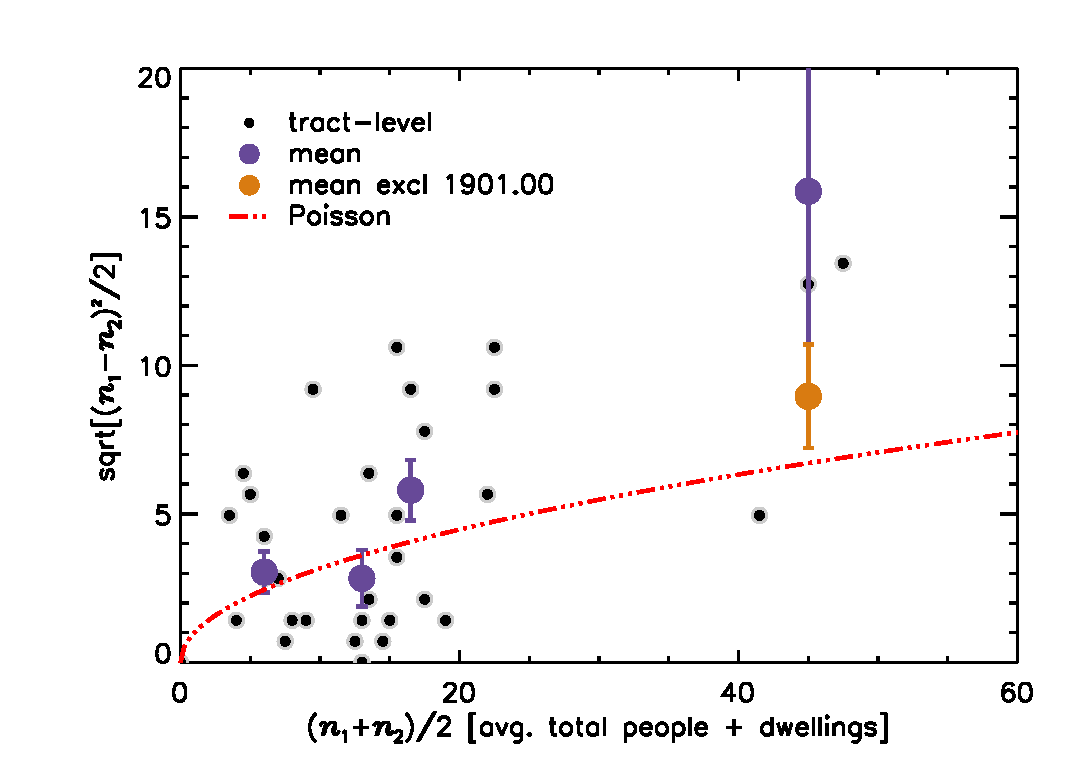
\includegraphics[width=\linewidth, trim = 1cm 0cm 0cm 0cm]{intDupeChar}\\
	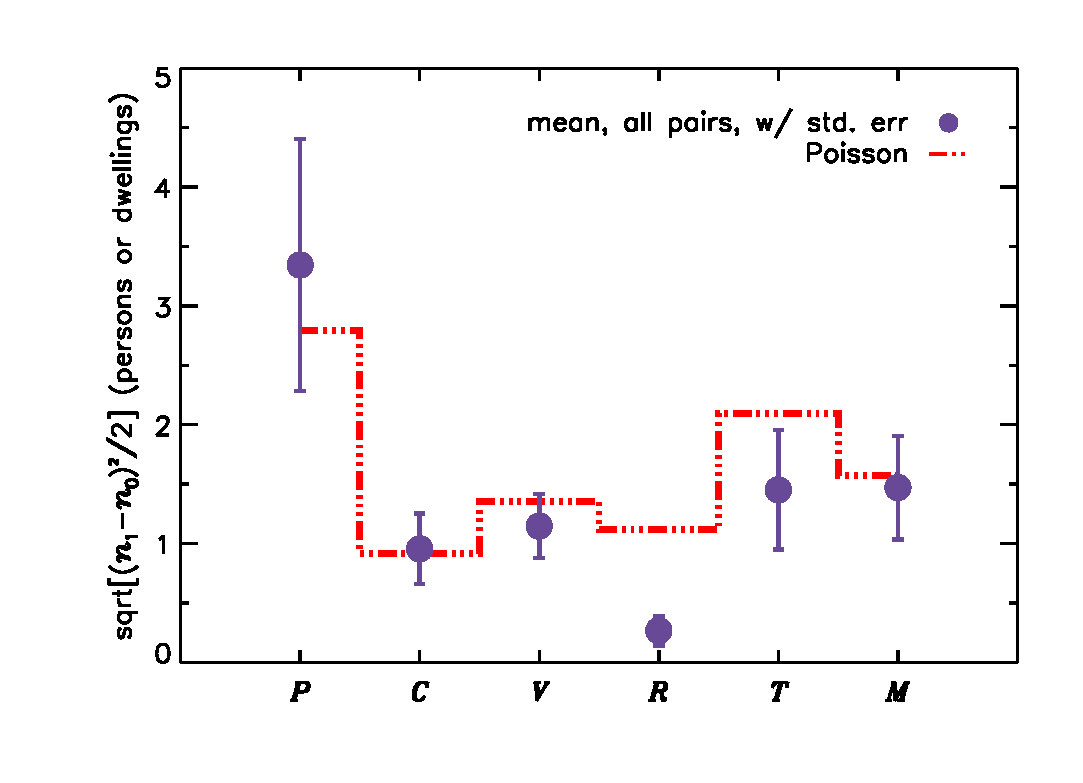
\includegraphics[width=\linewidth, trim = 1cm 0.5cm 0cm 0cm]{catDupeChar}
\caption{Duplicate tract (top) and category (bottom) count comparisons. Orange 
		points at top exclude tract 1901.00, which is a significant outlier.}
\label{fig:dupeChar}
\end{figure}
\subsubsection{Null Entries and Background Rates}
\label{sec:nulls}

Often, no persons or dwellings of a specific category are observed in a given census tract. Due to shot 
noise, however, these data are consistent with non-zero values for the true population. The Monte Carlo 
PDF reconstruction thus allows all such entries to take non-zero values based on an assumed background rate,
$\sigma_{j}^{\rm bkg}$. 

\begin{table*}[t]
\centering
\caption{Greater Hollywood 2021 PIT Unsheltered Data and Population Estimates}
%\resizebox{\linewidth}{!}{%
\begin{tabular}{lccccc}
\toprule
 & $C$ & $V$ & $R$ & $T$ & $M$ \\ \cmidrule{1-6}
{\bf SPA4/CD13} & $1.51\pm0.25$ & $1.77\pm0.42$ & $1.42\pm0.28$ & $1.48\pm0.11$ & $1.68\pm0.31$ \\
2021 $T$ & -- & -- & -- & $1.39\pm0.14$ & --\\
2021 $T$ w/ unocc & -- & -- & --& $1.51\pm0.24$ & --\\
%2021 $T$ & $1.51\pm0.25$ & $1.77\pm0.42$ & $1.42\pm0.28$ & $1.39\pm0.14$ & $1.68\pm0.31$\\
%2021 $T$ w/ modeled unocc & $1.51\pm0.25$ & $1.77\pm0.42$ & $1.42\pm0.28$ & $1.51\pm0.24$ & $1.68\pm0.31$\\
SPA4 & $1.38\pm0.11$ & $1.68\pm0.22$ & $1.32\pm0.15$ & $1.45\pm0.06$ & $1.64\pm0.16$\\
\bottomrule
\end{tabular}
%}
\caption*{CVRTM weights tested. Dashes denote identical values to the entry above. Bold denotes 
baseline scenario incorporating the 
\href{https://www.lahsa.org/documents?id=4635-usc-2018-2020-multipliers-and-estimates-overview}
{2020 SPA4/CD13 CVRTM weights} underpinning the latest official Hollywood and East Hollywood 
\href{https://www.lahsa.org/documents?id=4686-2020-greater-los-angeles-city-community-homelessness-report-service-planning-area-4.pdf}{Community Summaries}.}
\label{tbl:weights}
\end{table*}

Ideally, that rate would be based on category variations in similar tracts defined by some independent 
criteria. Sufficient data from, e.g., the US Census may enable such an exercise, but it is beyond the scope of 
this analysis. Instead, we adopt a noise floor based on the counts expected if all elements of a given category
were distributed evenly across all tracts. Hence:
\begin{equation}
	\sigma_{j}^{\rm bkg} \equiv \sqrt{\frac{1}{39}\sum_{\rm tracts}n_{j}},
\end{equation}
where $n_{j}$ are the raw counts in that category as defined in Equation \ref{eq:monte}.

While oversimplistic (Section \ref{sec:concentration}), this method works for any category, 
$j$, for which there is at least one individual/dwelling observed in any 
tract. However, for categories for which this is not the case---unaccompanied minors and families, in the
case of Hollywood---we set $\sigma_{j, \rm min}$ to the lowest non-zero value of the other categories
(corresponding to TAY). The adopted backgrounds are thus: 
\begin{equation}
	\sigma_{j,\, \rm min}=\{3.2, 0.4, 0.4, 0.9, 1.3, 1.1, 2.8, 2.5, 0.4\}
\end{equation}
adults, TAY, unaccompanied minors, cars, vans, RVs, tents, makeshifts, and families per tract. 

Note that the above numbers are not added to null entries, only random draws from normal distributions
of that width. This treatment is somewhat arbitrary, but we employ it symmetrically---per-tract category 
totals can be $<$0---so it does not bias the final inference. Instead, it sets the upper limits of intrinsically 
low-frequency categories and inflates aggregate uncertainties.

\begin{figure*}[t]
	\centering
	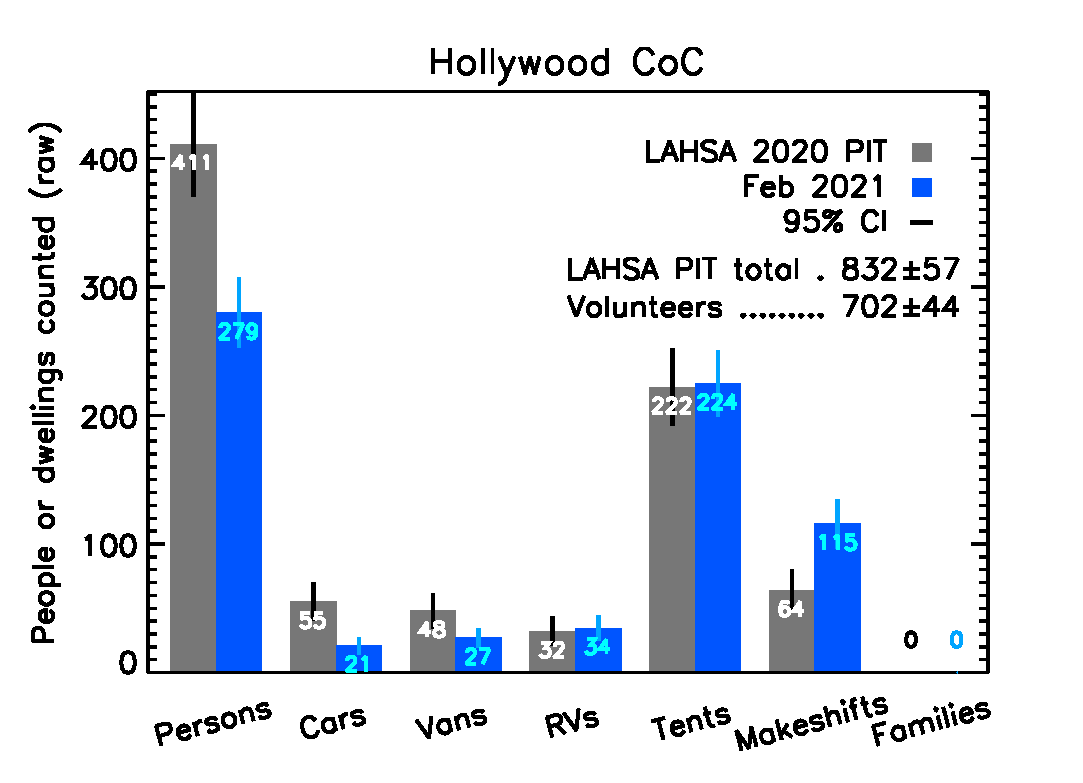
\includegraphics[width = 0.47\textwidth, trim = 1cm 0cm 0cm 0cm]{Hwood2021Bars}
	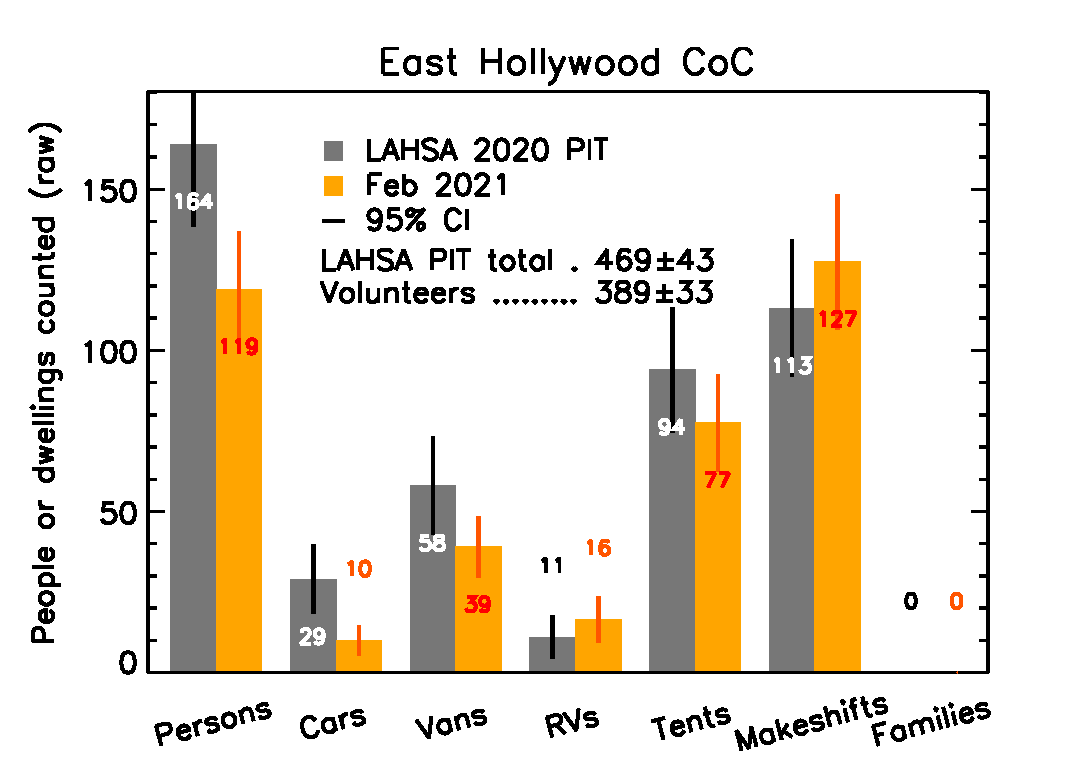
\includegraphics[width = 0.47\textwidth, trim = 0cm 0cm 1cm 0cm]{Eho2021Bars}
	\caption{Raw tallies of unsheltered persons and dwellings in Hollywood and East Hollywood
			(left/right) from the 2020 and 2021 PIT counts (grey/colors). Persons, cars, 
			and vans fell in both communities while RVs and tents stayed statistically flat. 
			Makeshift structures are the only category to show a potential common increase. 
			Overall, we identified 208 fewer people and dwellings compared to 2020,
			with similar 16\% decreases assessed by almost entirely independent teams
			in both communities. ``Persons'' are TAY+Adults.}
	\label{fig:rawCounts}
\end{figure*}

\begin{figure*}[t]
	\centering
	\includegraphics[width =0.47\linewidth, trim = 0.5cm 0cm 0cm 0cm]{hwoodHist}
	\includegraphics[width =0.47\linewidth, trim = 0cm 0cm 0.5cm 0cm]{ehoHist}
	\caption{Explain what the PDFs and CDFs are, what the colors mean.}
	\label{fig:communityPDFs}
\end{figure*}

\subsection{Duplicate Counts}
\label{sec:dupes}

Each volunteer tract in both communities (30) were assigned to at least two independent counting teams.
Four tracts additionally received a third pass. Pass 1 was organized numerically by tract number.
Pass 2 paired projected high-population tracts with a nearby tract. Pass 3 was the same as Pass 1 with 
tract pairings presented in reverse order (such that teams deployed simultaneously would likely start 
in different tracts). 

Results for one of the two teams assigned to tract 1925.20 could not be interpreted, making it the only
volunteer tract with one population estimate.

Figure \ref{fig:dupeChar} shows the intercounter comparisons of raw counts (people+dwellings)
at the tract and category levels. Average offsets are close to Poisson expectations in all cases 
except for the highest occupancy tracts, where they are inflated by an outlier (see below).
Explicitly, $\langle\sqrt{(n_{1}-n_{2})^{2}/(n_{1} + n_{2})}\rangle=1.4$, where
$n$ are the total raw counts of dwellings and people in a given tract returned by one of the teams. 

The outlier is tract 1901.00, whose repeat measurements differ by $6.6\sigma$. There, 
one team counted $\{P,C,V,R,T,M\}=\{23,1,1,1,6,2\}$ while the other counted $\{77,15,10,1,6,6\}$. 
Abramson re-counted this tract on-foot 14 hours after the PIT tally, obtaining $\{36, 4, 6, 0, 8, 2\}$.
In total, this tally ($56\pm7$) is within 1.9$\sigma$ of the mean of the two volunteer teams ($75\pm6$). 
As such, we treat the PIT entries identically to the rest.  As illustrated in Figure \ref{fig:dupeChar}, top,
the mean intercounter variance drops (to $1.3\,\sigma$) if this tract is excluded.

In terms of categories, all are consistent with Poisson expectations with the exception of RVs, on 
which agreement is significantly better. Given their salience, this finding is reassuring if also unsurprising.

%1901.00 inter-counter difference is 4.7 sigma (sqrt(delta) / root(n1 + n2) / root(2))

%\begin{itemize}
%%	\item All vol tracts counted at least twice;
%%	\item 4 tracts counted 3x;
%%	\item One recount DQed for quality flag (1925.20);
%%	\item Dupe statistics look pretty good. Mean abs discrepancy is consistent
%%		with zero given standard error on mean except for TAY (2.7 sigma) and RVs (3.8).
%%		Normalized differences ($|n_{1}-n_{2}|/\sqrt{n_{1}+n_{2}}$) are a little higher
%%		than $1\sigma$ ($CVRTM=[1.7, 1.1, -, 1.6, 1.4, 0.6, 1.2, 1.6, -]\sigma$), suggesting 
%%		a little more than poisson counting uncertainty, but LEA cross-checked the one
%%		highly discrepant ($\sim$8$\sigma$) tract, 1901.00, and found raw counts consistent
%%		with the average of the two nighttime datasets ($\sim$9:00 AM 26 Feb). 
%	\item Above holds true for 1912.01, which is in Hwood and also a SELAH recount tract. LEA
%		counted 51 totoal ppl/dwellings 12:30 P on 27 Feb vs 51 by vols night of count.
%\end{itemize}

No team counted tracts in both Hollywood and East Hollywood. As such, the volunteer counts
in those communities represent totally independent datasets. Once the professional-counted tracts are 
included, cross-talk comes only from one tract in East Hollywood counted by a team that surveyed five 
tracts in Hollywood. We discuss intercommunity comparisons between volunteer and professionally 
counted tracts in Section \ref{sec:comp}.

%{\bfr PRO TRACT RAW COUNT SHARE 2020: 44\% (23 tracts)
%
%PRO TRACT RAW COUNT SHARE 2021: 43\% (all tracts)}
%
%{\bfr Barely consistent if all of last year's vans and cars are still here. 95\% confidence limit $996\pm69$ can reach 1065 (v 1058) 
%in Hollywood, $598\pm 59= 657$ vs.\ 656 last yr in E.~Hollywood. BOTH AT 2020 SPA4 WEIGHTS!}


\section{Results}
\label{sec:results}

This section presents community level estimates for the number of unsheltered people living in
Hollywood and East Hollywood as of 25 February 2021. Sections \ref{sec:hWood} and \ref{sec:eHo} 
summarize our results; Section \ref{sec:comp} compares them to the 2020 LAHSA PIT estimates.

%Section \ref{sec:discussion} describes how 
%varying elements of Section \ref{sec:mc}'s analysis modulates these results.

\begin{table*}[t!]
\caption{Greater Hollywood 2021 PIT Unsheltered Data and Population Estimates}
\resizebox{\linewidth}{!}{%
\begin{tabular}{lcccccccccc}
\toprule
 & Adult & TAY & Car & Van & RV & Tent & Makeshift & {\bf 2021 Total} & {\bf 2020 Total} & {\bf Difference} \\ \cmidrule{1-11}
{\bf Hollywood} \\ %\cmidrule{1-1}
Counts & 277 & 2 & 21 & 27 & 34 & 224 & 115 & {\bf 702} & {\bf 831} & $\bf -15\%$ \\
Inhabitants & 277 (27) & 2 (5) & 32 (11) & 49 (13) & 50 (14) & 332 (29) & 195 (24) & {\bf 937 (93)} & {\bf 1058} & $\bf -11\%\,(9\%)$\\% (76)
Category share & 30\% (3\%) & 0\% (0\%) & 3\% (1\%) & 5\% (1\%) & 5\% (1\%) & 35\% (3\%) & 21\% (3\%) & -- & -- & -- \\ \cmidrule{1-11}
{\bf East Hollywood} \\ %\cmidrule{1-1}
Counts & 114 & 4 & 10 & 39 & 16 & 77 & 127 & {\bf 389} & {\bf 469} & $\bf -17\%$ \\
Inhabitants & 114 (19) & 4 (4) & 15 (8) & 70 (15) & 24 (9) & 115 (19) & 216 (23) & {\bf 557 (83)} & {\bf 656} & $\bf -15\%\,(12\%)$\\% (60)
Category share & 20\% (3\%) & 1\% (1\%) & 3\% (1\%) & 13\% (3\%) & 4\% (2\%) & 20\% (3\%) & 39\% (4\%) & -- & -- &--
\\ \bottomrule
\end{tabular}
}
\caption*{Parentheses denote 90\% uncertainties (binomial in the case of the categories). 
Uncertainties larger than estimates imply that only upper limits are available. Marginalized
upper limits are obtainable from the results file and imply $<$3 unaccompanied minors and
$<$3 unsheltered families in either community.}
\label{tbl:summary}
\end{table*}


\subsection{Hollywood}
\label{sec:hWood}

Counters identified $702\pm44$ (95\% CI) persons and dwellings in the 21 census tracts 
comprising the Hollywood community. Modulated by the baseline CVRTM weights, these 
estimates imply a total unsheltered population in Hollywood of $936\pm92$ people 
(90\% CI; Figure \ref{fig:communityPDFs}, left), with the plurality (35\%) living in tents 
(Table \ref{tbl:summary}; Figure \ref{fig:rawCounts}, left). The five tracts counted by professional 
teams---largely along the US 101 corridor---comprised 42\% of raw counts and 43\% of inferred 
unsheltered people. Tract 1910.00 (pro-counted) had the most people and dwellings (123); 
1899.03 had the fewest (0). These tracts also bracket the population statistics. 

Modifying the CVRTM weights from the baseline SPA4/CD13 values to the SPA4 wide values 
lowers Hollywood's inferred total unsheltered population to $912\pm68$ people; applying
an updated tent weight based on a survey in Hollywood raises it to $944\pm118$ people (Section
\ref{sec:discussion}). Neither represents a significant change from baseline.

\subsection{East Hollywood}
\label{sec:eHo}

Counters identified $389\pm33$ (95\% CI) persons and dwellings in the 18 census tracts 
comprising East Hollywood. Modulated by the baseline CVRTM weights, these estimates imply 
a total unsheltered population in East Hollywood of $556\pm83$ people (Figure \ref{fig:communityPDFs},
right), with the plurality (39\%) living in makeshift structures (Table \ref{tbl:summary}, 
Figure \ref{fig:rawCounts}, right). The four tracts counted by professional teams comprised 46\% of 
those counts and 47\% of inferred unsheltered people. Tract 1927.00 (pro-counted) had the 
most people and dwellings (87); 1912.04 had the fewest (5). These tracts also bracket the 
total population statistics. 
%The plurality of counts were of makeshift structures---statistically 
%consistent with the number of persons identified on the street---followed by tents 
%(Figure \ref{fig:rawCounts}, right).

Modifying the CVRTM weights from the baseline SPA4/CD13 values to the SPA4 wide values 
lowers East Hollywood's inferred total unsheltered population to $539\pm59$ people; applying
the updated tent weight raises it to $559\pm87$ people. Neither represents a significant change from 
baseline.

\begin{figure*}[]
	\centering
	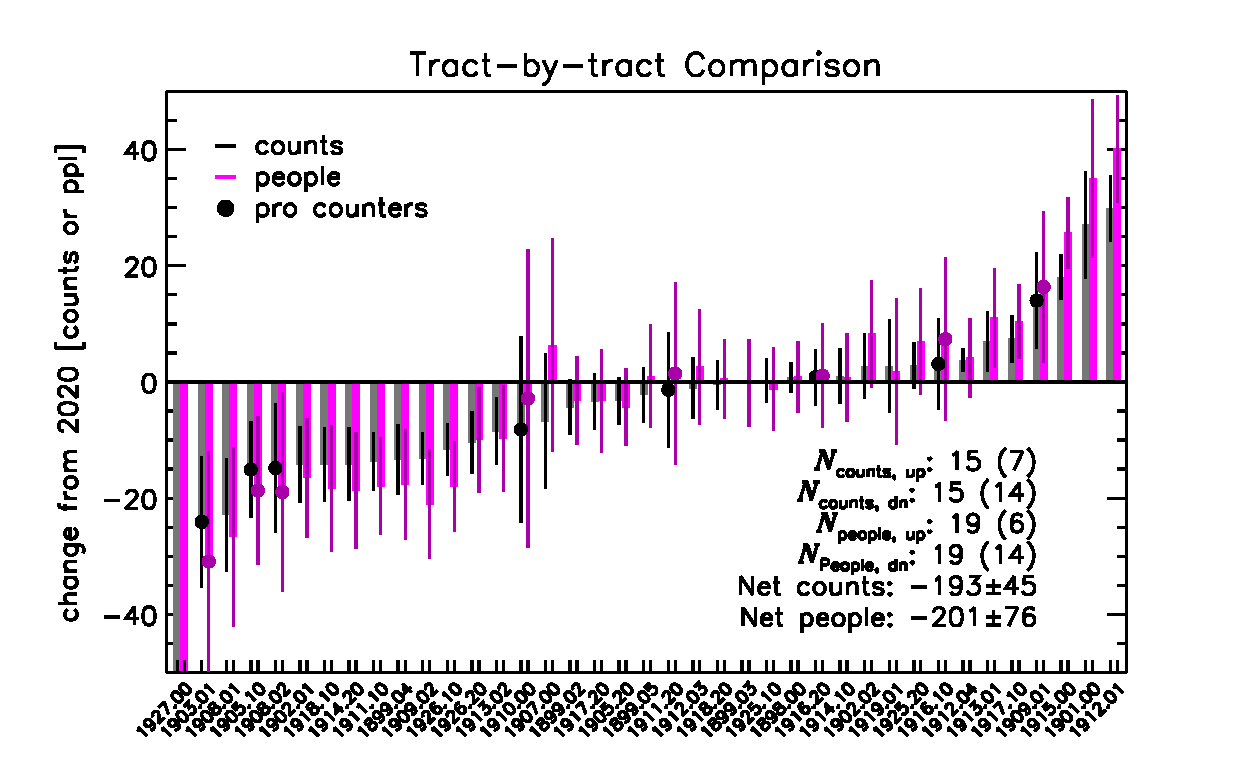
\includegraphics[width = 0.8\linewidth, trim = 0cm 0cm 0cm 0cm]{tractsYrYr}
	\caption{Tract-level year-on-year changes. Pro and vol trends are similar. Net loss of
			about 200 people or identified persons+structures. 1927.00 saw the biggest
			loss, which is explainable via XYZ.}
	\label{fig:tractYrYr}
\end{figure*}

\begin{figure*}[]
	\centering
	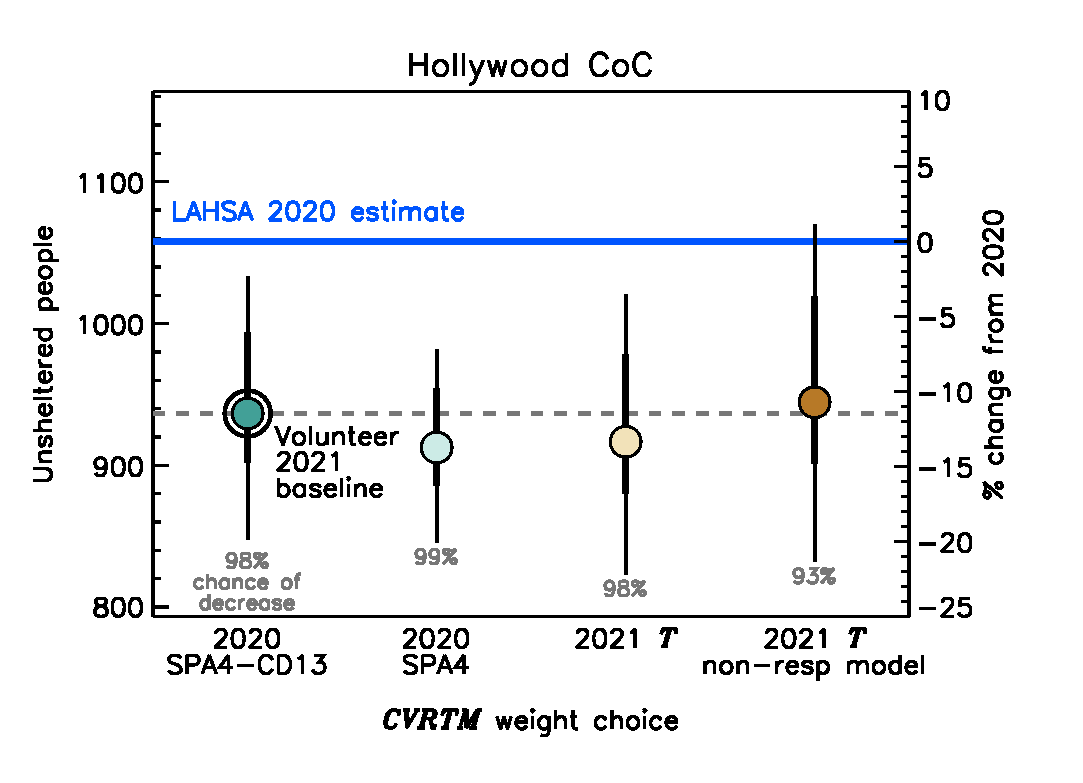
\includegraphics[width = 0.48\textwidth, trim = 0cm 0.5cm 0cm 0cm]{hwoodFinal}
	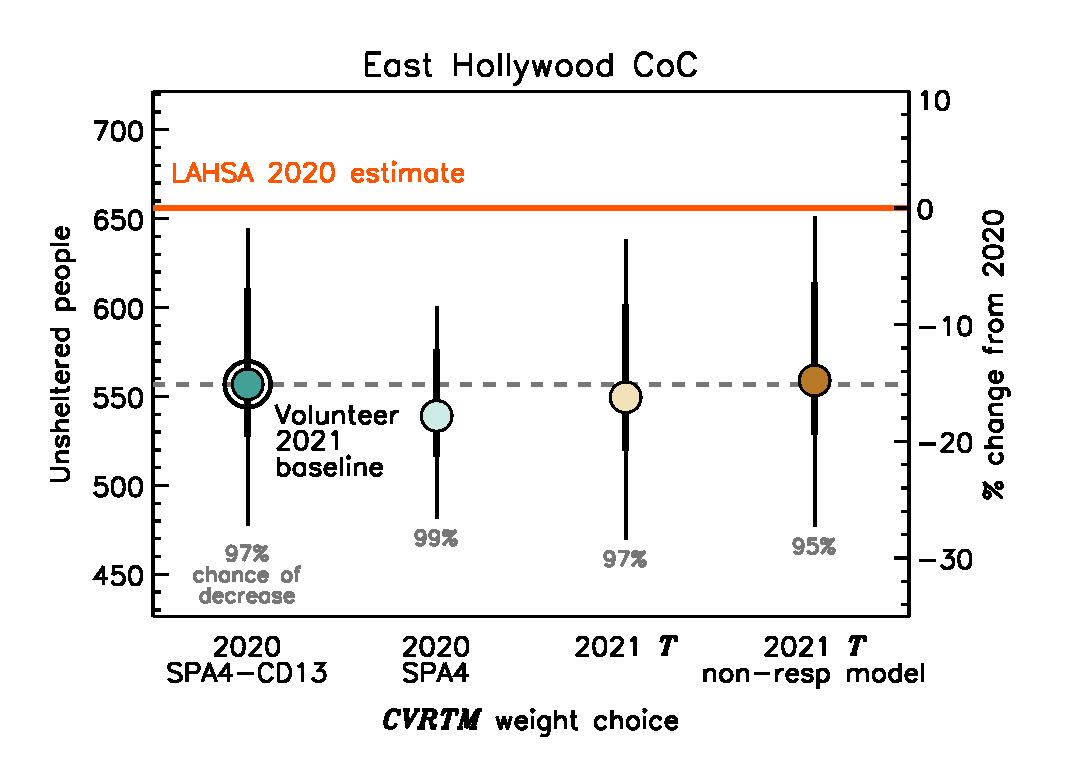
\includegraphics[width = 0.48\textwidth, trim = 0cm 0.5cm 0cm 0cm]{ehoFinal}	
	\caption{Unsheltered populations in Hollywood (left) and East Hollywood (right) 
			as functions of CVRTM weights. The baseline estimate uses the same weights as the 
			2020 LAHSA Community Summaries. Using SPA4 weights or replacing the tent 
			weight, $T$, with results from a survey conducted in Hollywood yields consistent
			results. All imply at least a 93\% chance that unsheltered homelessness has fallen
			by some amount, with likely declines of $12\%\pm9\%$ and $15\%\pm12\%$
			in Hollywood and East Hollywood, \resp.}
	\label{fig:wtComp}
\end{figure*}


%\begin{figure}[]
%	\centering
%	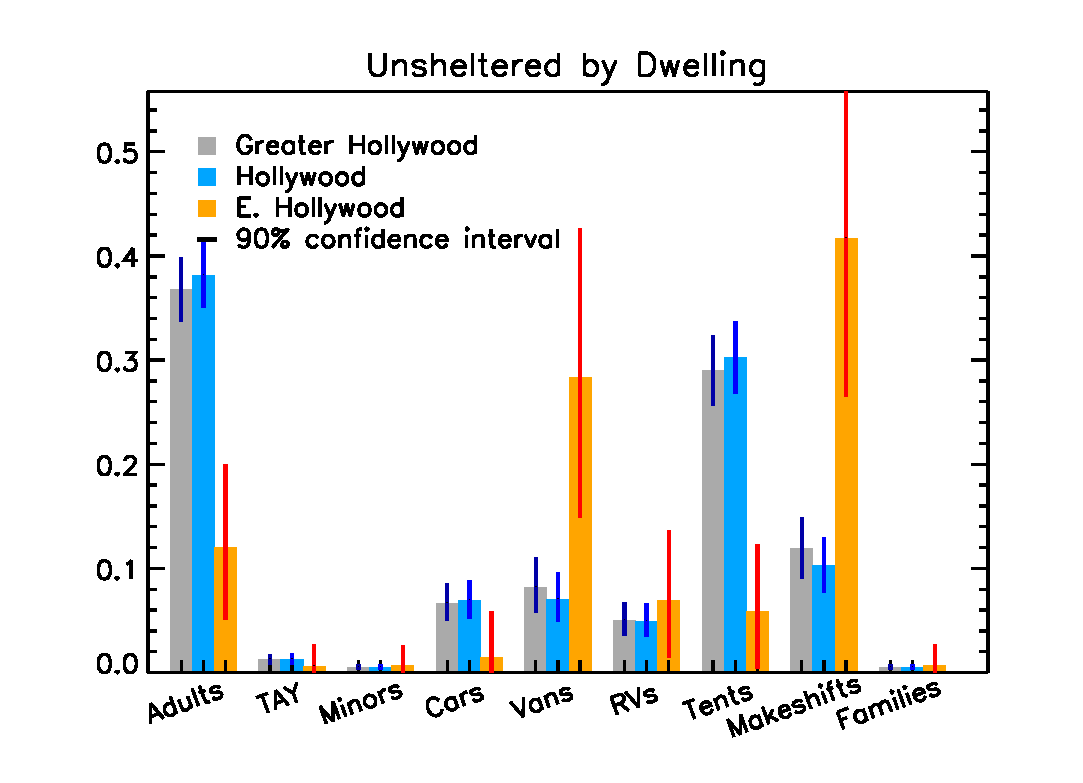
\includegraphics[width =\linewidth]{allTracts/allBreakdownBar}
%	\caption{}
%	\label{fig:popFracs}
%\end{figure}

\subsection{Comparison to 2020}
\label{sec:comp}

The official LAHSA estimates from the 2020 PIT count are overplotted in Figure \ref{fig:communityPDFs} 
as a red vertical line in each panel: 1058 unsheltered people in Hollywood, 656 in East Hollywood.
Our baseline inferences suggest a $>$95\% probability that the current population has fallen from 
those levels. Using the median and 90\% CI, we infer declines of $11\%\pm9\%$ and $15\%\pm12\%$, \resp. 

Figure \ref{fig:tractYrYr} shows the changes in counts and inferred population in each tract 
geographically illustrated in Figure \ref{fig:map}. In total, we find significant gains in 7 (6)
tracts in terms of counts (people), and significant declines in 14, resulting in net changes of $-193\pm45$
and $-201\pm76$ counts or people, \resp.\footnote{These estimates incorporate uncertainties 
from backing-out tract-level CVRTM counts from their total populations and person counts provided
by the LAHSA data portal.}

The tracts with the largest year-on-year gain (1912.01, $+40$ people) and loss (1927.00, $-125$ people)
are both in East Hollywood, and contain Barnsdall Park and US Rte.~101, \resp. 

%We speculate as to why these 
%tracts, specifically, saw such changes in Section \ref{sec:discussion}, along with why counts of rough
%saw particularly large declines.

Given the deficit in raw counts, it seems unlikely that reasonable modifications to the CVRTM weights 
will qualitatively change the trend we infer. The $T$ and $M$ weights are the largest potential error 
sources due to the high proportion of people living in tents and makeshifts. To constrain their evolution
from last year, \href{https://selahnhc.org}{SELAH} outreach teams surveyed 47 tents (38 responses) 
in Hollywood on 28 Feb. While the full 2021 PIT area has not been assessed, this exercise
yielding a mean occupancy of $T=1.39\pm0.14$ people per tent, or $T=1.50\pm0.22$ when 
non-responses are modeled.\footnote{We assumed they were equally likely to have anywhere 
from 0 to 4 occupants, each.} Although $M$ was not estimated, that $T$ value is consistent with 
the official 2020 weight of $T=1.48\pm0.11$. 

Figure \ref{fig:wtComp} illustrates the effect of the above CVRTM modifications, none of which 
alter our conclusions. In all cases, we infer at least a 93\% chance of a decline compared to the 2020 
PIT count.

While we encourage robust efforts to update the CVRTM weights, we caution that the changes needed 
to null the change we infer from 2020 are substantial. Only changes to $T$ and $M$ can achieve it, 
which must rise to 2.2 and 2.6 people from 1.5 and 1.7 people, \resp, in 2020. Not withstanding
the above survey, such $\sim$50\% increases in {\it mean} occupancies seem unlikely, especially as
known COVID-related tent distribution efforts have pushed in the opposite direction (Section 
\ref{sec:discussion}).

All of the above is in large part a reflection of the fact that a $\sim$30\% reduction in persons seen 
on the street drives the overall trend (Figure \ref{fig:rawCounts}). Cars and vans are also down from 
last year by more than the number of available safe parking spaces would suggest 
(Section \ref{sec:discussion}), but the total number of dwellings remained flat in most tracts. 
(Only makeshift structures show a potential common gain in both communities.)
Although uncertainties in East Hollywood are large, Figure \ref{fig:proVolComp} reveals these 
trends to be common to both communities and to tracts counted by volunteers or professionals.

Such consistencies in $\sim$independent datasets suggest the results are robust, and further 
cross-checks are presented in the next section.

%(Unsheltered people make up 3.5\% of tract 1907.00's total population, according to 2020 estimates
%from the US Census.)
%combined with COVID-related relaxations of tent-folding ordinances and the de-scoping of
%sanitation efforts suggests that the 

\begin{figure}[]
	\centering
	\includegraphics[width =\linewidth, trim=0.5cm 0cm 0cm 0cm]{volProfComp}
	\caption{Comparison of trends in pro- and vol-counted tracts in both communities.
			Consistency is good, though 1927.00 counts for a lot.}
	\label{fig:proVolComp}
\end{figure}

\subsection{Cross-checks}
\label{sec:crossChecks}

Four cross-checks involving independent counters and the use of external datasets validate the
results presented above by suggesting that the raw counts from our 2021 PIT \Count\ are accurate:

\subsubsection{Internal checks}

First, as shown in Figure \ref{fig:dupeChar}, inter-comparisons of the count's 37 duplicate tract 
measurements suggest per-tract and per-category counting uncertainties are consistent with the 
random errors built into the analysis. As such, there is no evidence that counters were biased in
their identification of unsheltered persons or dwellings. Such a statement does not preclude the
possibility that all teams were systematically blind, e.g., to cars and vans, we simply have no 
affirmative evidence to that effect.

However, the fact that trends hold in tracts counted by volunteers and professionals---who made 
their assessments on foot and in daylight---suggests that such biases are likely not to be large,
as do post-facto independent measurements of key geographies.

\subsubsection{External checks}

Six additional external checks also suggest our PIT enumerations are accurate.

First, three specific census tracts were re-surveyed in detail:
\begin{itemize}
	\item Tract 1901.00: the only outlier tract in terms of inter-counter variability. L.~Abramson
		  recounted this tract 14 hours after the PIT count (circa 9:00 AM) with results 
		  $1.9\sigma$ {\it below} the average of the volunteer teams' results.
	\item Tract 1912.01: the tract with the largest increase. L.~Abramson recounted this tract on 
		27 Feb.\ circa 12:00 PM with results consistent with the PIT teams' assessments
		to within $1\,\sigma$.
	\item Tract 1927.00: the tract with the largest decrease. L.~Abramson recounted this tract
		on 4 March circa 8:30 AM by vehicle with results lower than the PIT's assessment. 
		However, because this tract is especially dense and contains many freeway shoulders,
		it was originally surveyed on foot by outreach professionals. As such, the vehicular recount
		suggests that the PIT data are not biased in ways that would induce an artificial 
		year-on-dear decline.				
\end{itemize}

Two larger-geography surveys also concur:
\begin{itemize}
	\item Biweekly survey data from \href{https://hollywoodpartnership.com/}{\it The Hollywood Partnership} 
		from 19 Feb.\ are consistent with our PIT count in a common tract (1902.02) and with an independent 
		recount of that entire geography performed 28 Feb.\ by Abramson and Kohan. These also show 
		a decline from past values.
	\item Three tracts in Echo Park and Silver Lake monitored biweekly by SELAH since May 2020 
		also show similar declines to that implied by our data. 
\end{itemize}
%
%A 27 Feb.\ recount of tract 1912.01 in East Hollywood conducted as as part of a
%		\href{https://selahnch.org}{SELAH} monitoring campaign agrees with our PIT value.% in unsheltered homelessness.
%

Finally, safe parking---a known sink---seems unable to account for sufficient cars and vans
to meaningfully affect our conclusions. 49 spaces exist in or near the survey area (Hollywood,
East Hollywood, and Echo Park). These probably did go uncounted, and may have been occupied 
by $80\pm16$ total car and van dwellers ($1\,\sigma$, assumes equal mix). If so, the chance of a 
decline from 2020 falls from 98\% to 92\% in the baseline case. 

All of the above suggests that our results are quantitatively and qualitatively reliable.
%Assumes equal mix of cars + vans.
%From Starkey: Hwood = 25, Eho = 10, EchoPk = 14; total = 49; total CD13 = 59 but I think it's reasonable
%to truncate at Echo Pk. It's 90% if you include all 59 spaces.

%		   P	C     V	    R	 T     M
%1901.00 -- 50    8    5.5   1     6      4 -- 2021, raw
%1901.00 -- 36    4     6     0     8      2 -- 26 Feb ABRAMSON 9.00 AM
%
%1927.00 -- 48    1      5     0    53    70 -- 2020, raw
%1927.00 -- 20    0     0     7     6     54 -- 2021, raw
%1927.00 -- 15     0     9     5    14    21 -- 4 Mar 2021 ABRAMSON 8.45 AM
%
%1912.01 --  18.5  0.5  3.5  1.5  5.5  12 -- 2021, raw
%1912.01 --  21     0      4     1     8      6  -- 27 Feb ABRAMSON 12.15 PM
%
%1902.02 -- 9      --     --     --     8   5.5 -- 2021, raw
%1902.02 -- 9      --     --     --    17    --  -- BID 2/19

% 1907.00 is also interesting in that total population stayed nearly the same but identified
% individuals and dwellings basically swapped: IND 73->38; CVRTM 31->70. This has a big impact
% on people's perceptions, and it's in a very high-traffic part of the community.

%The pro/vol trends are consistent everywhere except tract 1927.00, 
%			where pro counts dropped significantly more for both individuals and dwellings (esp.\ 
%			tents). 1927.00 comprises 22\% of total counts in East Hollywood. Unsheltered 
%			homelessness in that CoC was flat or rose slightly outside of that tract.}
%{\bfr 1927.00 is the tract with the PATH Madison PSH. Phase II opened in Jan 2020---leasing began May 
%2020---and is 120 units, some of which were filled from nearby folks but I dunno how many. LEA recounted 
%this tract 4 March at $\sim$9:00 AM and found 94 total population vs.\ pro's 129. Only place where
%LEA counted more objects was vans. Adding that to the pro total adds 16 people (9 vans).

%HOLLYWOOD -- Zero delta requires CVRTM mean occupancies of:\\
% - 5.00 ppl/car (from 1.51)\\
% - 5.00 ppl/van (from 1.77)\\
% - 4.95 ppl/RV (from 1.42)\\
% - 2.03 ppl/tent (from 1.48)\\
% - 2.73 ppl/mkshft (from 1.68)\\
%
%EAST HOLLYWOOD -- Zero delta requires CVRTM mean occupancies of:\\
% - 5.00 ppl/car (from 1.51)\\
% - 4.33 ppl/van (from 1.77)\\
% - 5.00 ppl/RV (from 1.42)\\
% - 2.78 ppl/tent (from 1.48)\\
% - 2.45 ppl/mkshft (from 1.68)

% ------ SUMMARY for HWOOD ------ 
%
%Total People (90%CI) .   936+/-92
%Fraction vs. last yr .   0.89+/-0.09
%Total counts..........   702
% > Adults    : 277 (39%), 277, (29%)
% > TAY       :   2 ( 0%),   2, ( 0%)
% > Minors    :   0 ( 0%),   0, ( 0%)
% > Cars      :  21 ( 2%),  31, ( 3%)
% > Vans      :  27 ( 3%),  47, ( 5%)
% > RVs       :  34 ( 4%),  49, ( 5%)
% > Tents     : 224 (31%), 330, (35%)
% > Makeshifts: 115 (16%), 193, (20%)
% > Families  :   0 ( 0%),   0, ( 0%)
%% Compiled module: MINMAX.
%Min/max ppl/tract ..... 0, 169
%Min/max counts/tract .. 0, 123
%
% ------ SUMMARY for EHO ------ 
%
%Total People (90%CI) .   556+/-83
%Fraction vs. last yr .   0.85+/-0.13
%Total counts..........   389
% > Adults    : 114 (29%), 114, (20%)
% > TAY       :   4 ( 1%),   4, ( 0%)
% > Minors    :   0 ( 0%),   0, ( 0%)
% > Cars      :  10 ( 2%),  14, ( 2%)
% > Vans      :  39 (10%),  68, (12%)
% > RVs       :  16 ( 4%),  23, ( 4%)
% > Tents     :  77 (19%), 114, (20%)
% > Makeshifts: 127 (32%), 214, (38%)
% > Families  :   0 ( 0%),   0, ( 0%)
%Min/max ppl/tract ..... 6, 129
%Min/max counts/tract .. 5, 87

\section{Discussion}
\label{sec:discussion}

If the global picture is one of a general decline in unsheltered population, smaller scales tell different 
stories. Seven tracts saw at least a 50\% increase in their number of dwellings; five saw more than 100\% 
gains.\footnote{Tracts 1902.02, 1907.00, 1912.01, 1915.00, 1925.20, which together account for nearly 
10\% of all identified street dwellings and 17\% of all counts.} 
In one case---tract 1907.00---the total population stayed nearly identical while the fraction of rough sleepers
and persons in CVRTM dwellings swapped (Figure \ref{fig:1907}). Given this tract's location---Fountain
to Sunset to Franklin, Vine to Highland to La Brea; the commercial heart of Central Hollywood---this
phenomenon might increase the {\it visual salience} of unsheltered living even as the population as a 
whole has declined. 

The lack of change in tents is notable as it suggests that known tent distribution efforts by 
providers must in large part have gone to replacing damaged or destroyed structures, at least 
in Greater Hollywood.

%Ancillary data from regularly monitored census tracts suggests that the date offset is unlikely to substantially 
%erode comparability between this and past datasets. Limited daytime recounts also suggest that 
%time-of-day effects are sub-dominant.

A $\sim$30\% drop in unsheltered individuals in both Hollywood and 
East Hollywood drives the decline we find, for which government initiatives to move people indoors 
(Project Roomkey) and staunch inflow into homelessness (eviction moratoria) may be responsible. 
Indeed, \href{https://www.lahsa.org/documents?id=4672-2020-homeless-count-council-district-13}{CD13's} share of \href{https://www.lahsa.org/documents?id=4585-2020-greater-los-angeles-homeless-count-los-angeles-continuum-of-care-coc-}{LA County's unsheltered senior population} (6.5\%) implies that perhaps 100 of its \href{https://projectroomkeytracker.com/}{1608 occupied rooms} were filled with Greater Hollywood residents on the night 
of the count---about half the inferred change. The opening of at least one 
\href{https://www.lamayor.org/ABridgeHome}{\it A Bridge Home} site in Los Feliz---whose catchment area 
includes Greater Hollywood---and 120 PATH permanent supportive housing units may also have contributed. 
The latter are located in tract 1927.00. While all of those units did not go to local residents, any that did would help
drive that tract's large observed decrease. Coordinated Entry System data will constrain these possibilities.
%1927.00 is actually in the catchment of 3 ABHs that were either new or expanded between PIT counts. 
%Lodi, however, did not fill its new beds, and Lafayette doesn't cover the whole tract, so we won't speculate.
%Nevertheless, technically, even at 50\% decompression, residents of 1927.00 may have been eligible 
%for any of 89 new ABH beds. It's also on the CoC boundary.

{\it However}, to say nothing of the implications of the above for conditions after the eviction moratoria
lapse, if there are fewer people on the street today, their quality of life has degraded markedly. COVID has restricted or 
eliminated access to restaurant and park bathrooms, libraries (and so 
\href{https://www.lapl.org/homeless-resources/the-source}{\it The Source} service days), DPSS 
(EBT, Medi-Cal), DMV (ID replacement), and DMH facilities. Physical limitations on caseworker 
access to clients at hospitals and clinics has also hindered successful discharges. These qualitative harms are reflected 
by a 25\% increase in 
\href{https://www.latimes.com/california/story/2021-01-07/the-powerful-synthetic-opioid-fentanyl-is-behind-rising-deaths-in-the-homeless-population}{overdose deaths}, and visually amplified by a doubling of unsheltered dwellings in 13\% of census 
tracts\footnote{Including 1907.00, Central Hollywood's commercial core.} as enforcement of tent folding ordinances
(LAMC 56.11) and City and State sanitation programs were simultaneously 
\href{https://clkrep.lacity.org/onlinedocs/2020/20-0147_misc_3-17-20_p.pdf}{suspended or de-scoped}. 
So, while the PIT data may support the efficacy of programs designed to reduce street 
homelessness, they do {\it not} suggest that the state of homelessness in Greater Hollywood has improved. In the 
fight to rebuild lives---as well as build homes---that fact must remain paramount.

\begin{figure}[]
	\centering
	\includegraphics[width =\linewidth, trim = 0.5cm 0cm 0cm 0cm]{tract1907comp}
	\caption{Illustration of what's happened in 4 tracts---persons and structures
			swapping prominence---in this case with the total population
			$\sim$conserved. This is also an example of one of 5 tracts where
			dwelling frequencies at least doubled. 1907 happens to be in the 
			heart of Central Hollywood, increasing the visual impact of this
			rise in dwellings.}
	\label{fig:1907}
\end{figure}

PRK effects.

ABH effects.

PSH effects.

{\bfr 1907.00 people and tents switched. Total unsheltered $\sim$constant but visual perceptions
in this most-highly trafficked tract will make it *feel* like homelessness has increased by a lot.}


Edges.

Deaths (COVID $\sim$300; \href{http://publichealth.lacounty.gov/phcommon/public/media/mediapubhpdetail.cfm?prid=2900#:~:text=LOS\%20ANGELES\%20\%E2\%80\%93The\%20Los\%20Angeles,deaths\%20among\%20people\%20experiencing\%20homelessness.}{ODs}...at least 6x higher
than that?).

\subsection{Concentration}
\label{sec:concentration}

\begin{figure}[]
	\centering
	\includegraphics[width =\linewidth, trim = 0cm 0cm 3.5cm 0cm]{gini}
	\caption{All tracts in Greater Hollywood. This Gini Coefficient
			is about the same as 
			\href{https://en.wikipedia.org/wiki/List_of_countries_by_income_equality}{Kenya's}.
			50\% of unsheltered persons and dwellings are concentrated in 20\% of census
			tracts.}
	\label{fig:gini}
\end{figure}


\section{Summary}
\label{sec:summary}

\section*{}

{\bfr Acknowledge Kelson}

\appendix

\section{Example Documents}

\begin{figure*}
	\centering
	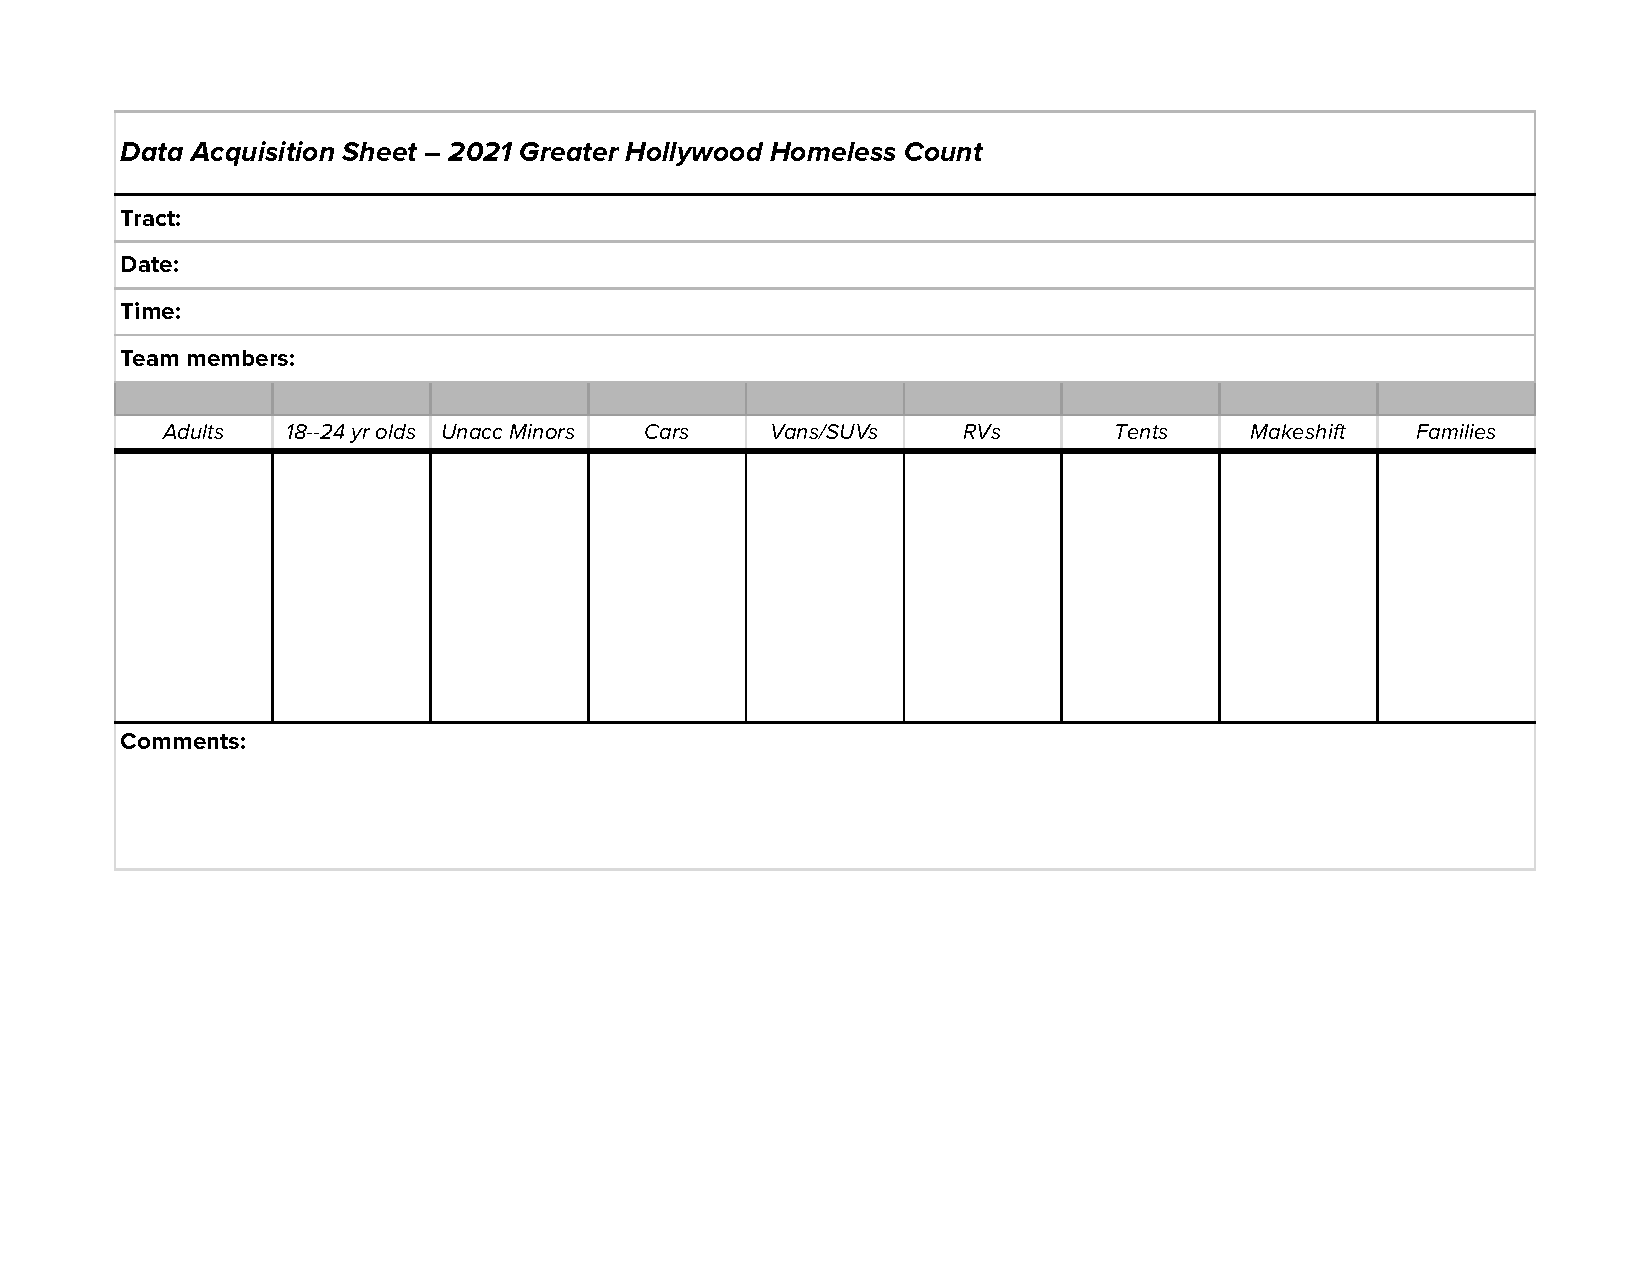
\includegraphics[width =\linewidth]{Hollywood2021CountDataSheet}
	\caption{Counter tally-sheet}
\end{figure*}

\begin{figure*}
	\centering
	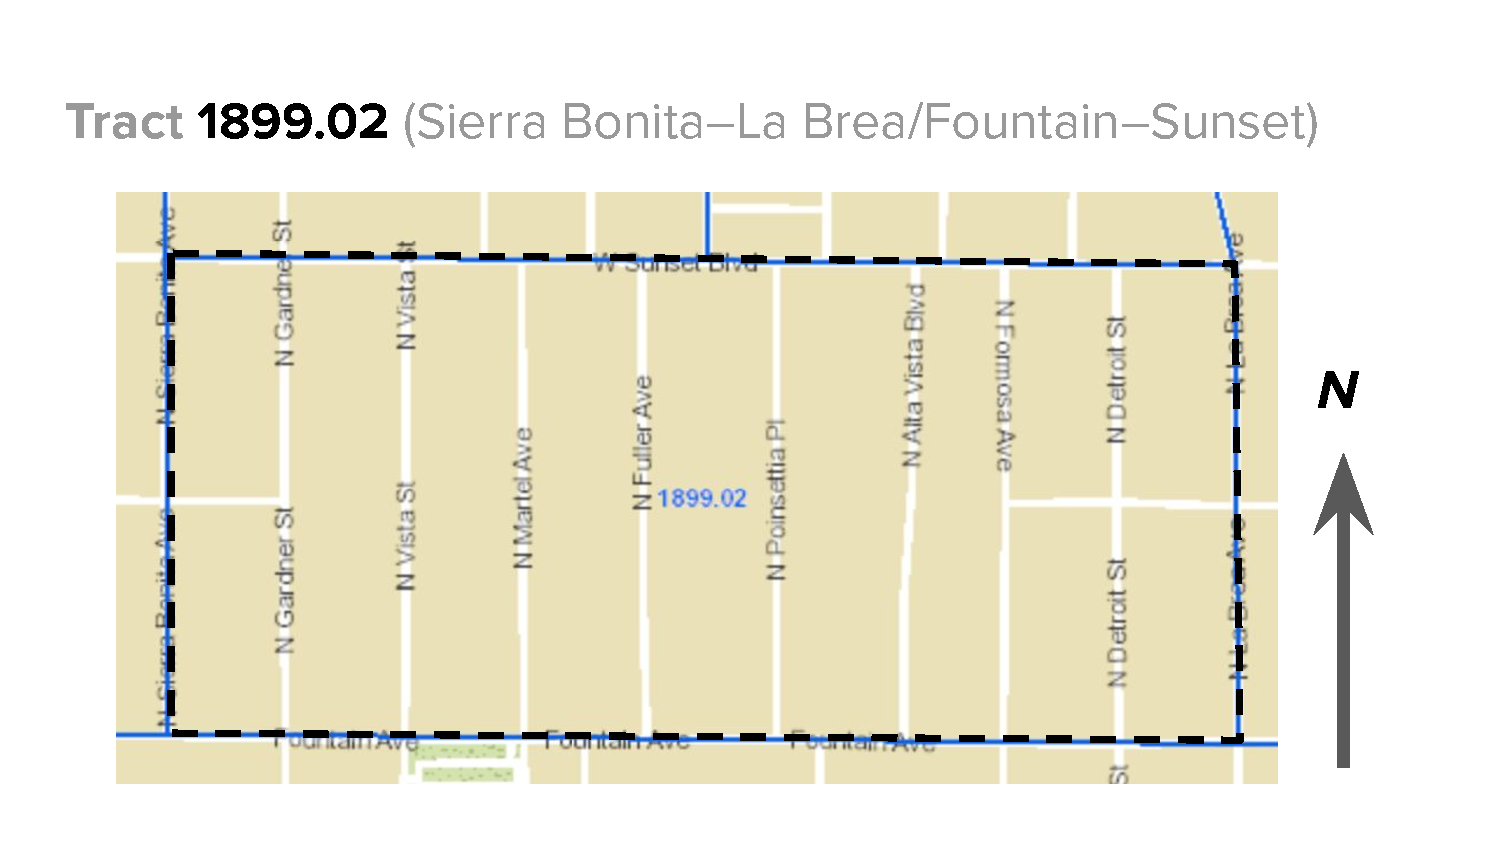
\includegraphics[width =\linewidth]{tractMap}
	\caption{Example Hollywood tract map.}
\end{figure*}

\begin{figure*}
	\centering
	\includegraphics[width =0.7\linewidth]{primerFront}
	\caption{Count primer {\bfr SCRUB EK'S NUMBER!}}
\end{figure*}

\section{Full Tract-level Results}

\begin{table*}[]
\caption{Census Tract-level Unsheltered Counts}
%\resizebox{\textwidth}{!}{%
\centering
\begin{tabular}{cccccccccc}
\toprule
Tract & Community & Counter & $A$ & {\it TAY} & $C$ & $V$ & $R$ & $T$ & $M$ \\ \cmidrule{1-10}
1898.00 & Hollywood & Vol &  3.3 &  0.3 &  0.0 &  0.7 & 0 &  1.3 &  0.0 \\
1899.02 & Hollywood & Vol &  4.3 &  0.0 &  0.0 &  1.3 & 2 &  4.0 &  1.3 \\
1899.03 & Hollywood & Vol &  0.0 &  0.0 &  0.0 &  0.0 & 0 &  0.0 &  0.0 \\
1899.04 & Hollywood & Vol &  9.5 &  0.0 &  0.0 &  1.0 & 0 &  2.5 &  2.0 \\
1899.05 & Hollywood & Vol &  3.0 &  0.0 &  3.0 &  4.5 & 1 &  2.0 &  0.0 \\
1901.00 & Hollywood & Vol & 49.5 &  0.5 &  8.0 &  5.5 & 1 &  6.0 &  4.0 \\
1902.01 & Hollywood & Vol & 14.5 &  0.0 &  0.5 &  0.0 & 0 &  2.5 &  1.5 \\
1902.02 & Hollywood & Vol &  9.0 &  0.0 &  0.0 &  0.0 & 0 &  8.0 &  5.5 \\
1903.01 & Hollywood & Pro & 10.0 &  0.0 &  0.0 &  0.0 & 0 & 19.0 & 22.0 \\
1905.10 & Hollywood & Pro & 13.0 &  0.0 &  0.0 &  0.0 & 4 &  6.0 &  4.0 \\
1905.20 & E.~Hollywood & Vol &  2.0 &  0.5 &  0.5 &  1.0 & 0 &  4.0 &  1.0 \\
1907.00 & Hollywood & Vol & 38.5 &  0.0 &  2.0 &  0.0 & 0 & 38.5 &  7.0 \\
1908.01 & Hollywood & Vol & 18.5 &  0.0 &  0.5 &  0.0 & 0 & 19.5 &  9.0 \\
1908.02 & Hollywood & Pro & 22.0 &  0.0 &  0.0 &  1.0 & 5 & 13.0 & 13.0 \\
1909.01 & Hollywood & Pro & 15.0 &  0.0 &  0.0 &  0.0 & 0 & 17.0 &  9.0 \\
1909.02 & Hollywood & Vol &  2.7 &  0.3 &  0.7 &  1.7 & 0 &  0.0 &  0.0 \\
1910.00 & Hollywood & Pro & 34.0 &  0.0 &  1.0 &  0.0 & 5 & 60.0 & 23.0 \\
1911.10 & E.~Hollywood & Vol &  4.0 &  0.5 &  0.0 &  0.0 & 0 &  2.5 &  0.5 \\
1911.20 & E.~Hollywood & Pro & 14.0 &  0.0 &  0.0 &  0.0 & 0 & 24.0 & 10.0 \\
1912.01 & E.~Hollywood & Vol & 17.5 &  1.0 &  0.5 &  3.5 & 1 &  5.5 & 12.0 \\
1912.03 & E.~Hollywood & Vol &  5.0 &  0.0 &  2.0 &  8.0 & 0 &  0.0 &  2.5 \\
1912.04 & E.~Hollywood & Vol &  3.0 &  0.5 &  0.5 &  1.0 & 0 &  0.0 &  0.0 \\
1913.01 & E.~Hollywood & Vol &  8.0 &  0.0 &  0.5 &  7.5 & 0 &  5.0 &  1.0 \\
1913.02 & E.~Hollywood & Vol &  5.5 &  0.0 &  0.5 &  0.5 & 0 &  3.5 &  6.0 \\
1914.10 & E.~Hollywood & Vol &  7.5 &  0.0 &  1.0 &  0.5 & 0 &  1.0 &  5.5 \\
1914.20 & E.~Hollywood & Vol &  4.0 &  0.0 &  2.0 &  4.5 & 1 &  3.0 &  2.0 \\
1915.00 & E.~Hollywood & Vol & 10.0 &  0.0 &  0.0 &  4.5 & 2 &  2.5 &  2.5 \\
1916.10 & E.~Hollywood & Pro &  6.0 &  0.0 &  0.0 &  1.0 & 1 &  2.0 & 22.0 \\
1916.20 & E.~Hollywood & Pro &  0.0 &  2.0 &  0.0 &  0.0 & 0 &  4.0 &  6.0 \\
1917.10 & Hollywood & Vol &  6.5 &  0.0 &  2.0 &  4.5 & 1 &  1.0 &  0.5 \\
1917.20 & Hollywood & Vol &  2.3 &  0.0 &  0.3 &  1.3 & 6 &  0.0 &  4.3 \\
1918.10 & Hollywood & Vol &  3.5 &  0.0 &  1.0 &  1.5 & 1 & 10.0 &  0.0 \\
1918.20 & Hollywood & Vol &  2.5 &  1.0 &  0.0 &  2.5 & 2 &  1.5 &  2.0 \\
1919.01 & Hollywood & Vol & 16.0 &  0.0 &  2.0 &  1.5 & 5 & 13.0 &  7.5 \\
1925.10 & E.~Hollywood & Vol &  4.0 &  0.0 &  1.5 &  1.0 & 1 &  0.0 &  1.5 \\
1925.20 & E.~Hollywood & Vol &  1.0 &  0.0 &  1.0 &  6.0 & 1 &  0.0 &  0.0 \\
1926.10 & E.~Hollywood & Vol &  2.0 &  0.0 &  0.0 &  0.0 & 0 &  3.5 &  0.5 \\
1926.20 & E.~Hollywood & Vol &  1.0 &  0.0 &  0.0 &  0.0 & 0 & 11.0 &  0.5 \\
1927.00 & E.~Hollywood & Pro & 20.0 &  0.0 &  0.0 &  0.0 & 7 &  6.0 & 54.0 \\
\bottomrule
\end{tabular}
%}
\caption*{Raw counts from each tract. Coding as in Table \ref{tbl:tractStats}. Fractional counts
reflect averages over multiple counters.}
\label{tbl:allCount}
\end{table*}

\begin{table*}[]
\caption{Census Tract-level Unsheltered Population Inferences}
\resizebox{\linewidth}{!}{
\begin{tabular}{cccccccccc}
\toprule
Tract & Community & Counter & $A$ & {\it TAY} & $C$ & $V$ & $R$ & $T$ & $M$ \\ \cmidrule{1-10}
1898.00 & H & V &  3.3 ( 1.7) &  0.9 ( 0.6) &  2.3 ( 2.2) &  2.8 ( 1.5) &  2.8 ( 2.8) &  1.9 ( 1.6) &  7.0 ( 7.0)  \\
1899.02 & H & V &  4.3 ( 2.0) &  0.7 ( 0.7) &  2.3 ( 2.3) &  2.3 ( 2.2) &  3.8 ( 2.5) &  5.9 ( 2.9) &  2.2 ( 2.0)  \\
1899.03 & H & V &  5.2 ( 5.2) &  0.7 ( 0.7) &  2.2 ( 2.2) &  3.9 ( 3.9) &  2.8 ( 2.8) &  6.8 ( 6.8) &  7.0 ( 7.1)  \\
1899.04 & H & V &  9.5 ( 3.6) &  0.7 ( 0.7) &  2.2 ( 2.3) &  4.1 ( 2.2) &  2.7 ( 2.7) &  3.7 ( 2.7) &  3.3 ( 3.0)  \\
1899.05 & H & V &  3.0 ( 2.0) &  0.7 ( 0.7) &  4.4 ( 3.3) &  7.7 ( 5.4) &  3.3 ( 1.7) &  2.9 ( 2.5) &  7.2 ( 7.1)  \\
1901.00 & H & V & 49.5 ( 8.2) &  1.3 ( 0.8) & 11.8 ( 5.9) &  9.5 ( 6.1) &  3.3 ( 1.8) &  8.9 ( 4.3) &  6.6 ( 4.5)  \\
1902.01 & H & V & 14.5 ( 4.4) &  0.7 ( 0.7) &  2.1 ( 1.3) &  4.0 ( 3.9) &  2.8 ( 2.8) &  3.7 ( 2.8) &  5.2 ( 2.5)  \\
1902.02 & H & V &  9.0 ( 3.5) &  0.7 ( 0.7) &  2.2 ( 2.2) &  4.0 ( 4.0) &  2.8 ( 2.8) & 11.8 ( 5.0) &  9.1 ( 5.3)  \\
1903.01 & H & P & 10.0 ( 5.2) &  0.7 ( 0.7) &  2.2 ( 2.2) &  3.9 ( 3.9) &  2.7 ( 2.7) & 27.8 (11.0) & 36.5 (16.8)  \\
1905.10 & H & P & 12.9 ( 5.9) &  0.7 ( 0.7) &  2.3 ( 2.2) &  3.9 ( 4.0) &  5.7 ( 5.1) &  8.8 ( 6.0) &  6.5 ( 5.9)  \\
1905.20 & E & V &  2.0 ( 1.6) &  1.3 ( 0.8) &  2.1 ( 1.3) &  4.2 ( 2.2) &  2.8 ( 2.8) &  5.9 ( 3.6) &  3.9 ( 2.1)  \\
1907.00 & H & V & 38.5 ( 7.2) &  0.7 ( 0.7) &  3.0 ( 2.6) &  3.8 ( 3.9) &  2.8 ( 2.8) & 56.7 (12.8) & 11.6 ( 6.3)  \\
1908.01 & H & V & 18.5 ( 4.9) &  0.7 ( 0.7) &  2.1 ( 1.3) &  3.9 ( 3.9) &  2.7 ( 2.8) & 28.6 ( 8.4) & 14.9 ( 7.4)  \\
1908.02 & H & P & 21.9 ( 7.7) &  0.7 ( 0.7) &  2.2 ( 2.2) &  5.0 ( 3.1) &  7.1 ( 5.8) & 19.0 ( 9.1) & 21.3 (11.8)  \\
1909.01 & H & P & 15.0 ( 6.3) &  0.7 ( 0.7) &  2.3 ( 2.3) &  4.0 ( 4.0) &  2.8 ( 2.8) & 24.9 (10.6) & 14.8 ( 9.4)  \\
1909.02 & H & V &  2.7 ( 1.5) &  0.9 ( 0.6) &  2.2 ( 1.2) &  2.9 ( 2.5) &  2.7 ( 2.7) &  6.8 ( 6.8) &  7.2 ( 7.2)  \\
1910.00 & H & P & 34.0 ( 9.6) &  0.7 ( 0.7) &  4.1 ( 2.6) &  4.0 ( 3.9) &  7.0 ( 5.7) & 88.1 (21.7) & 38.1 (17.4)  \\
1911.10 & E & V &  4.0 ( 2.3) &  1.3 ( 0.8) &  2.2 ( 2.2) &  3.9 ( 3.9) &  2.8 ( 2.7) &  3.6 ( 2.8) &  2.3 ( 1.4)  \\
1911.20 & E & P & 13.9 ( 6.1) &  0.7 ( 0.7) &  2.2 ( 2.2) &  3.9 ( 3.9) &  2.8 ( 2.7) & 35.3 (12.8) & 16.4 (10.1)  \\
1912.01 & E & V & 17.5 ( 4.9) &  2.1 ( 1.1) &  2.1 ( 1.3) &  6.0 ( 4.6) &  4.5 ( 2.2) &  8.1 ( 4.2) & 19.9 ( 9.0)  \\
1912.03 & E & V &  5.0 ( 2.6) &  0.7 ( 0.7) &  3.0 ( 2.6) & 13.9 ( 7.8) &  2.7 ( 2.8) &  6.8 ( 6.8) &  4.2 ( 3.3)  \\
1912.04 & E & V &  3.0 ( 2.0) &  1.3 ( 0.8) &  2.1 ( 1.3) &  4.2 ( 2.2) &  2.8 ( 2.8) &  6.7 ( 6.8) &  7.0 ( 7.0)  \\
1913.01 & E & V &  8.0 ( 3.3) &  0.7 ( 0.7) &  2.1 ( 1.3) & 13.0 ( 7.5) &  2.0 ( 1.2) &  7.3 ( 3.9) &  3.8 ( 2.0)  \\
1913.02 & E & V &  5.5 ( 2.7) &  0.7 ( 0.7) &  2.1 ( 1.3) &  2.5 ( 1.5) &  2.0 ( 1.2) &  5.1 ( 3.2) &  9.9 ( 5.6)  \\
1914.10 & E & V &  7.5 ( 3.2) &  0.7 ( 0.7) &  3.4 ( 1.8) &  2.6 ( 1.6) &  2.7 ( 2.8) &  3.2 ( 1.7) &  9.0 ( 5.3)  \\
1914.20 & E & V &  4.0 ( 2.3) &  0.7 ( 0.7) &  3.0 ( 2.7) &  7.7 ( 5.3) &  3.3 ( 1.8) &  4.4 ( 3.0) &  3.3 ( 3.0)  \\
1915.00 & E & V & 10.0 ( 3.6) &  0.7 ( 0.7) &  2.2 ( 2.2) &  7.8 ( 5.3) &  3.5 ( 2.9) &  3.7 ( 2.7) &  4.1 ( 3.4)  \\
1916.10 & E & P &  6.0 ( 4.0) &  0.7 ( 0.7) &  2.3 ( 2.3) &  5.0 ( 3.1) &  4.0 ( 2.4) &  6.5 ( 3.4) & 36.4 (16.9)  \\
1916.20 & E & P &  5.2 ( 5.2) &  4.3 ( 2.3) &  2.3 ( 2.3) &  3.9 ( 3.9) &  2.8 ( 2.8) &  5.8 ( 4.9) & 10.0 ( 7.5)  \\
1917.10 & H & V &  6.5 ( 3.0) &  0.7 ( 0.7) &  3.0 ( 2.6) &  7.8 ( 5.4) &  3.3 ( 1.7) &  3.3 ( 1.8) &  2.3 ( 1.4)  \\
1917.20 & H & V &  2.3 ( 1.5) &  0.7 ( 0.7) &  1.4 ( 0.9) &  2.3 ( 2.1) &  9.0 ( 4.3) &  6.6 ( 6.8) &  7.1 ( 3.9)  \\
1918.10 & H & V &  3.5 ( 2.2) &  0.7 ( 0.7) &  3.4 ( 1.8) &  5.6 ( 2.7) &  4.4 ( 2.2) & 14.6 ( 5.7) &  7.0 ( 6.9)  \\
1918.20 & H & V &  2.5 ( 1.8) &  2.2 ( 1.2) &  2.2 ( 2.3) &  4.3 ( 3.8) &  2.9 ( 2.6) &  2.2 ( 2.1) &  3.3 ( 3.0)  \\
1919.01 & H & V & 16.0 ( 4.7) &  0.7 ( 0.7) &  2.9 ( 2.6) &  5.6 ( 2.7) &  7.1 ( 4.3) & 19.1 ( 6.6) & 12.4 ( 6.5)  \\
1925.10 & E & V &  4.0 ( 2.3) &  0.7 ( 0.7) &  4.7 ( 2.2) &  4.2 ( 2.2) &  4.5 ( 2.2) &  6.7 ( 6.7) &  5.3 ( 2.6)  \\
1925.20 & E & V &  2.6 ( 1.6) &  0.7 ( 0.7) &  4.1 ( 2.5) & 10.5 ( 8.3) &  3.9 ( 2.4) &  6.8 ( 6.8) &  7.1 ( 7.1)  \\
1926.10 & E & V &  2.0 ( 1.6) &  0.7 ( 0.7) &  2.2 ( 2.3) &  4.0 ( 4.0) &  2.8 ( 2.8) &  5.1 ( 3.3) &  2.3 ( 1.4)  \\
1926.20 & E & V &  2.2 ( 1.2) &  0.7 ( 0.7) &  2.2 ( 2.2) &  3.9 ( 4.0) &  2.8 ( 2.8) & 16.1 ( 6.1) &  2.3 ( 1.4)  \\
1927.00 & E & P & 19.9 ( 7.4) &  0.7 ( 0.7) &  2.3 ( 2.3) &  3.9 ( 3.9) & 10.0 ( 7.0) &  8.8 ( 6.0) & 90.4 (33.2)\\ 
\bottomrule
\end{tabular}
}
\caption*{Median and 90\% CI listed.}
\label{tbl:allPop}
\end{table*}

%\begin{table*}[]
%\caption{Tract 1898.00 Unsheltered Data}
%\resizebox{\linewidth}{!}{%
%\begin{tabular}{lcccccccccc}
%\toprule
% & Adult & TAY & Unacc Minor & Car & Van & RV & Tent & Makeshift & Family & {\bf Total} \\ \cmidrule{1-11}
%Counts & 3 & 0 & 0 & 0 & 0 & 0 & 1 & 1 & 0 & {\bf 5} \\
%Inhabitants & 3 (3) & 0 (1) & 0 (1) & 1 (2) & 1 (2) & 1 (2) & 2 (2) & 2 (2) & 0 (1) & {\bf 9 (6)} \\
%Category share & 0.31 (0.29) & 0.03 (0.10) & 0.03 (0.10) & 0.09 (0.18) & 0.10 (0.19) & 0.07 (0.16) & 0.16 (0.23) & 0.18 (0.24) & 0.03 (0.10) & - 
%\\ \bottomrule
%\end{tabular}
%}
%\caption*{Quantities in parentheses denote 95\% uncertainties (binomial in the case of the categories). Uncertainties larger than estimates imply that only upper limits can be stated confidently.}
%\label{tbl:}
%\end{table*}

\end{document}  